% Shared main-matter body for kbound_short.tex (IEEEtran) and kbound_tmlr.tex (article/TMLR).
% Runs from \section{Introduction} through the Conclusion. Front matter (title, author,
% abstract, keywords) and back matter (appendix, bibliography) live in the driver files.
\section{Introduction}\label{sec:intro}
\begin{figure}[t]\centering
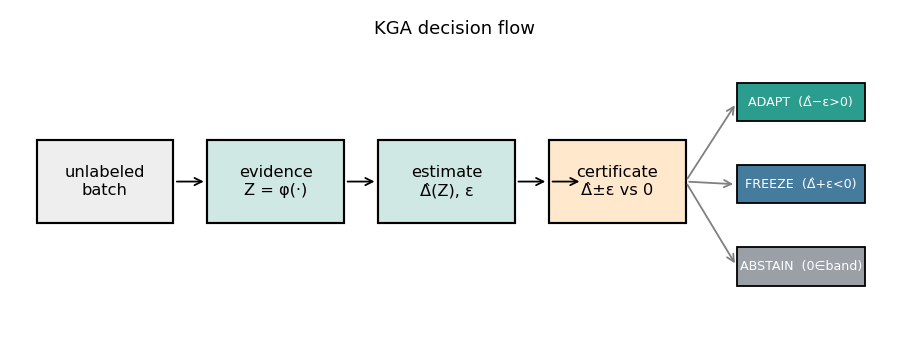
\includegraphics[width=0.86\columnwidth]{figures/fig_decision_flow.png}
\caption{\textbf{K-Bound previews the decision.} From an unlabeled batch under shift, the certificate
estimates the adaptation benefit $\widehat\Delta$ with a finite-sample radius $\varepsilon$ and returns
\textsc{adapt} (certified helpful), \textsc{freeze} (certified harmful), or \textsc{abstain} (no
supported strict commitment). Under interval coverage it controls the marginal events
$\Pr(\textsc{adapt},\Delta\le0)$ and $\Pr(\textsc{freeze},\Delta\ge0)$ at level $\alpha$; no
conditional-error guarantee is claimed.}
\label{fig:teaser}
\end{figure}
Test-time adaptation (TTA) updates a model on the unlabeled test stream and, under favorable
distribution shift, recovers accuracy. Under unfavorable shift, the same objective silently
degrades it, and with no target labels the system usually cannot tell which case it faces.
The decision that matters therefore comes \emph{before} the update: given a frozen
baseline $f_0$ and an adapted candidate $f_a$, choose
\textbf{adapt} when adaptation is knowably helpful, \textbf{freeze} when knowably harmful, or
\textbf{abstain} when label-free evidence cannot identify the sign of the benefit. The field's
default assumption is that adaptation should be made robust enough to always run; we replace it
with an explicit, certified decision about whether to run it at all.

Some cases are information-theoretically unknowable. It is established that label-free
quantities cannot decide adaptation without an assumption on the shift: identifying OOD
accuracy is as hard as identifying the optimal predictor~\cite{garg2022atc}, and the optimal
predict-versus-abstain rule under a shift budget has a known form~\cite{kalai2021abstain}. We
localize this landscape to the paired benefit sign. The load-bearing step is a construction: for any
margin strictly inside the declared band there are two admissible target laws whose label-free
evidence laws are \emph{identical} and whose benefits have opposite nonzero signs
(Theorem~\ref{lem:nonid}), which forces abstention at rate $\ge1-2\alpha$ on that evidence fibre
(Corollary~\ref{cor:matched-abstain}); on the boundary, zero-versus-strict ambiguity still rules out a
uniformly sound strict action (Proposition~\ref{prop:closed-band}). Packaging this with the
observable/latent split $\Delta\leftrightarrow M+\gamma$---a definitional decomposition, not a derived
one (Remark~\ref{rem:gamma-residual})---gives the strict-commitment criterion
$|M|>\beta$ (Theorem~\ref{thm:headline}), whose sufficiency half is interval arithmetic and whose
necessity half is the construction. The same construction shows that $\beta$ itself admits no
non-vacuous label-free audit (Appendix~\ref{app:audit-short}), which is why K-Bound treats the budget
as declared. \textsc{KGA}
(Algorithm~\ref{alg:kga}) wraps a benefit estimator and a conformal radius around any
adapter (Tent, EATA, SAR). It realizes the three-way decision as a finite-sample certificate---a direct benefit estimate with a calibrated radius, not a numerical $|M|{>}\beta$ test---and controls
marginal false-adapt and false-freeze events under interval coverage (Theorem~\ref{thm:certificate}).

The evidence follows the regime map in Table~\ref{tab:regime-summary}, and the primary finding is a
safety one. On the four one-sided natural tracks with locked held-out artifacts---hospital
(Camelyon17), wildlife-camera (iWildCam), laboratory-batch (RxRx1), and domain (Office-Home)
shifts---KGA is \emph{no-harm}: it ties the better fixed policy and averts the failure of the wrong
one, with zero observed false adaptation, and it abstains rather than overclaim where the evidence is
weak. On the remaining three natural tracks the outcome is different and we report it as such: PACS is
a conservative null in which \textsc{KGA}'s mean regret ($0.0431$) is $2.45\times$ always-adapt's
($0.0176$); ImageNet-R is a weak-evidence null in which \textsc{KGA} ($0.0151$) is worse than
always-adapt ($0.0064$) on $7$ of $10$ backbones; and CIFAR-10.1 fails the declared transfer bar at
$\mathrm{FA}_{\mathrm u}=0.167$. No-harm is therefore a claim about the one-sided locked tracks, not a
universal property of the panel. Where it does hold it is the contribution, not a shortfall: a valid
label-free certificate cannot beat a fixed policy that is already optimal, so tying it while avoiding
the opposite failure is exactly correct behavior. A three-way router can beat both fixed policies only
where helpful and harmful conditions coexist and the evidence separates them, in the operational sense
defined in \S\ref{sec:detectability}; we report those beats-both results as secondary mechanism
confirmation, on stress and constructed regimes only, never as single-dataset natural-shift dominance.
K-Bound therefore provides a safety, validity, and abstention layer for TTA rather than an accuracy
boost, and does not claim universal improvement.

\paragraph{Plain-language takeaway.}
The question that matters at deployment is not how hard to adapt but whether to adapt at all. K-Bound
answers it with a certificate: adapt only when label-free evidence certifies benefit, freeze when it
certifies harm, and \textsc{abstain} otherwise (the maximal sound three-way rule when
$|M|\le\beta$; KGA implements the distinct finite-sample interval decision). On the one-sided natural-shift
datasets this returns \emph{no-harm}---safety or abstention---which is exactly the point; on the
domain-generalization and rendition tracks it returns a conservative null that costs regret relative
to always-adapt, and we report that too. Beating both fixed policies additionally requires a mixed
regime the evidence can separate (\S\ref{sec:detectability}) and is reported as a secondary check,
with any constructed pooled mixture labeled as such, never as single-dataset natural-shift dominance.

\paragraph{Contributions.}
\begin{enumerate}
\item \textbf{TTA as a safety decision.} We recast test-time adaptation as a pre-commitment \emph{whether-to-adapt} problem---adapt, freeze, or abstain---and make the target risk difference, fallback semantics, and target-label-free information boundary explicit. The object of study is the validity of the decision, not the accuracy of the adapter.
\item \textbf{A matched-evidence impossibility construction, and the vacuity of label-free budget audits.} We exhibit two target laws inside the declared class whose label-free evidence laws are \emph{equal}---not merely close---and whose benefits have opposite nonzero signs (Theorem~\ref{lem:nonid}), and we show that abstention is forced at rate $\ge 1-2\alpha$ on that fibre (Corollary~\ref{cor:matched-abstain}). The same label-kernel construction yields the result with the most operational content in the paper: any label-free audit $\widehat\beta$ that is valid uniformly over the unrestricted class must return $\widehat\beta\ge\tfrac12+|M|$, so the audited frontier abstains in every world (Theorem~\ref{thm:short-audA}). This is why the drift budget in K-Bound is \emph{declared} rather than estimated, and it is a statement no amount of better label-free evidence can repeal.
\item \textbf{A bookkeeping decomposition and the frontier it induces.} Splitting the disagreement-region accuracy into an observable margin $M$ and a latent calibration drift $\gamma$ gives $\sign\Delta=\sign(M+\gamma)$ (Lemma~\ref{lem:reduction}). We state plainly what this is: $\gamma$ is \emph{defined} as the residual $\bar a-\tfrac12-M$, so the decomposition is an identity and the sufficiency half of Theorem~\ref{thm:headline} ($|M|>\beta\Rightarrow\sign\Delta=\sign M$) is interval arithmetic on $[M-\beta,M+\beta]$. Its value is organizational---it names the quantity a deployment must bound---and the mathematical content of Theorem~\ref{thm:headline} lies entirely in the necessity clause, which rests on the construction above.
\item \textbf{Coverage-based false-adapt certificate.} Under measurable interval coverage, the finite-sample rule controls the marginal false-adapt and false-freeze rates at level $\alpha$ (Theorem~\ref{thm:certificate})---the deployable safety guarantee. We do not claim this interval construction as novel machinery; it is split-conformal-style calibration applied to a paired benefit, and its contribution is the decision object it is attached to.
\item \textbf{KGA deployable wrapper.} KGA wraps Tent/EATA/SAR without changing their adaptation objectives and uses shadow state, commit, rollback, and logging (Algorithm~\ref{alg:kga}). It is adapter-interface agnostic but adapter-specific in calibration: the benefit model and radius are refit per dataset and per candidate adapter.
\item \textbf{Scoped no-harm evidence, with the negatives kept.} A pre-registered nine-track panel shows KGA is no-harm on the four one-sided natural tracks with locked held-out artifacts, abstains under weak evidence, and beats both fixed policies only on stress and constructed regimes that meet the ex ante detectability criterion of \S\ref{sec:detectability}. Honest nulls and failures (PACS, ImageNet-R, CIFAR-10.1) are retained and reported with the direction of loss, and the one track where the guarantee is actually exercised at power (CIFAR-10-C, $1{,}113$ adapts, $0$ false) is separated from the tracks where an observed $\mathrm{FA}_{\mathrm u}=0$ is uninformative (Table~\ref{tab:decision-accounting}). Fixed-policy regret comparisons are a secondary routing-utility check.
\end{enumerate}

\begin{table}[t]\centering\footnotesize
\caption{\textbf{Regime map: expected behavior vs.\ result.} Each regime, an example dataset, the
behavior the frontier predicts for a valid certificate, and what was measured. ``No-harm'' means
matching the better fixed policy while avoiding the worse; comparisons with both fixed policies are
secondary routing-utility diagnostics. The evidence tier in Table~\ref{tab:uniform-panel}
states whether that point verdict is locked, reconciled, provisional, or diagnostic. Regime
assignment follows Definition~\ref{def:detectable}, applied before outcomes are read.}
\label{tab:regime-summary}
\begin{tabular}{@{}p{0.19\linewidth}p{0.24\linewidth}p{0.22\linewidth}p{0.25\linewidth}@{}}
\toprule
Regime & Example & Expected & Result \\
\midrule
Helpful-dominated & Camelyon17 OOD & tie always-adapt & no-harm, but not reproducible from release \\
Harmful-dominated & RxRx1; iWildCam/Office-Home (OOF lock) & tie always-freeze, beat always-adapt & locked no-harm; $0$/$1$/$22$ adapts \\
Domain-gen.\ natural & PACS (4 LODO splits) & no-harm or abstain & \textbf{null; loses to always-adapt} $2.45\times$ \\
Mixed + detectable & CIFAR-10-C Tent/EATA & adapt helpful, freeze harmful, abstain near zero & locked; $0$ false adapts in $2357$; CI utility vs.\ both \\
Mixed, \emph{not} detectable & ImageNet-C Tent ($56\%$ harmful) & abstain / tie freeze & ties freeze; $0$ adapts \\
Weak evidence & ImageNet-R, CIFAR-10.1 & abstain / conservative & \textbf{diagnostics; ImageNet-R loses to always-adapt on $7/10$ backbones, CIFAR-10.1 fails the bar} \\
Constructed mixture & three-source OOF stream & route per condition & locked routing result, not transfer \\
\bottomrule
\end{tabular}
\end{table}

\noindent\emph{Table note.} The uniform panel below is the sole empirical index; diagnostic variants
and historical runs are not additional evidence for the headline claims.

\section{Related Work}\label{sec:related}
The closest literature improves test-time updates, monitors adaptation failures, estimates target performance without labels, or characterizes abstention under shift. K-Bound differs in the decision object: it certifies the sign of the frozen-versus-adapted risk difference before the candidate state is committed.

\subsection{Test-Time Adaptation}
Tent~\cite{wang2021tent}, SHOT~\cite{liang2020shot}, TTT~\cite{sun2020ttt}, EATA~\cite{niu2022eata}, SAR~\cite{niu2023sar}, CoTTA~\cite{wang2022cotta}, and MEMO~\cite{zhang2022memo} improve adaptation through entropy minimization, filtering, regularization, sharpness-aware updates, or temporal stabilization (survey:~\cite{liang2025ttasurvey}). These methods primarily answer \emph{how} to adapt. Even when the update rule is more stable, the deployment system generally still commits to adaptation rather than certifying that the candidate has positive target benefit.

\subsection{Guarded and Monitored Adaptation}
POEM~\cite{bar2024poem}, sequential risk monitors~\cite{schirmer2025monitoring,podkopaev2022tracking}, PeTTA~\cite{hoang2024petta}, and sample-level filters such as DeYO~\cite{lee2024deyo} guard an adaptation stream during or after updating; reset-timing rules for long-horizon streams~\cite{lim2026reset} decide when to \emph{restart} adaptation once it has already run. These approaches are complementary to K-Bound. They typically monitor a proxy or intervene in one failure direction, whereas K-Bound poses a pre-commitment three-way decision over the benefit sign and explicitly represents an unknowable region.

\subsection{Label-Free Performance Estimation}
ATC~\cite{garg2022atc}, agreement-on-the-line~\cite{baek2022aol,miller2021aol}, AETTA~\cite{lee2024aetta}, and related confidence-style estimators~\cite{deng2023confidence,xie2024mano} estimate target accuracy or error without target labels. Estimating $R_T(f)$ is not identical to certifying $\sign(R_T(f_0)-R_T(f_a))$: a deployment controller needs the sign of a paired risk difference and must account for uncertainty around zero. K-Bound uses this difference as the estimand and abstains when the available evidence does not identify its sign.

\subsection{Impossibility, Abstention, and Risk Control}
General label-free target-risk identification requires assumptions on the shift~\cite{garg2022atc,steinhardt2016,bendavid2010theory,rosenfeld2023dis2}. Kalai and Kanade~\cite{kalai2021abstain} characterize a related abstain-versus-predict decision under a shift budget, while selective prediction~\cite{geifman2017selective}, Chow's reject option~\cite{chow1970reject}, and learning-to-defer / reject-option classification~\cite{cortes2016boosting,madras2018learntodefer} abstain on individual labels. Its empirical uncertainty layer connects to split conformal prediction, conformal under shift, RCPS, and Learn-then-Test~\cite{tibshirani2019conformal,gibbs2021adaptive,barber2023beyond,bates2021rcps,angelopoulos2025ltt}.

\paragraph{Relation to classical DA and label-shift non-identifiability.}
Theorem~\ref{lem:nonid} constructs two target laws with identical unlabeled observables and opposite
label-dependent functionals. That is structurally the same move as the classical impossibility
results for domain adaptation~\cite{bendavid2010theory,bendavid2012hardness} and the identification
arguments underlying label-shift estimation~\cite{lipton2018bbse,garg2020labelshift}, and we do not
claim the move as new. Three things are specific to our setting. (i) The estimand is a \emph{paired
sign} $\sign(R_T(f_0)-R_T(f_a))$, not a risk level: it survives any monotone recalibration that
preserves the disagreement-region ordering, so estimator-quality arguments do not dispose of it.
(ii) The ambiguity is localized to the disagreement region $D$, which shrinks the construction from
the full risk range to a band of width $2\beta$ on a single conditional expectation. (iii) The class
is parameterized by a \emph{declared} budget, which turns an all-or-nothing impossibility into a
frontier with an operational knob --- and, by Aud-A (App.~\ref{app:audit-short}), a knob that cannot
be set from unlabeled data. Readers from the label-shift literature should read
Theorem~\ref{lem:nonid} as a localization of a known phenomenon, and Aud-A as the part that is not
already implied by it.

\subsection{Surviving Gap, and What Is Not Ours}
Existing work provides stronger adapters, reactive monitors, label-free accuracy estimates, and general abstention theory. The remaining gap is a pre-commitment rule for the sign of adaptation benefit that (i) distinguishes helpful, harmful, and unsupported decisions, (ii) states the assumptions under which the decision is valid, and (iii) controls marginal false adaptation under a calibrated uncertainty model. K-Bound addresses this gap with the population frontier and its finite-sample realization, \textsc{KGA}.

We state the other half explicitly, because it is easy to overstate. The interval machinery is
\emph{not} our contribution: confidence-sequence and anytime-valid risk monitoring for adaptation
streams already exists~\cite{schirmer2025monitoring,podkopaev2022tracking,bar2024poem}, and the
unsupervised-accuracy-estimation literature already states the no-assumption impossibility
informally~\cite{garg2022atc}. Our certificate shares machinery with that line; what we add is the
pre-commitment decision object, the explicit abstention region, and the accounting of when the
resulting guarantee is actually tested --- not the interval construction.

\section{Problem Formulation and Validity}\label{sec:setup}

\subsection{Deployment Setting and Adaptation Benefit}
Source data follow $P_S(X,Y)$ and may be labeled during training and development. Deployment data follow $P_T(X,Y)$, but only target inputs and model outputs are available when the decision is made. A frozen predictor $f_0$ serves as the safe fallback, and an adapter $\mathcal A$ proposes a temporary candidate $f_a=\mathcal A(f_0,X_{1:m})$ from an unlabeled target batch. For loss $\ell$, the target risk and adaptation benefit are
\begin{equation}
R_T(f)=\E_{P_T}[\ell(f(X),Y)],\qquad
\Delta=R_T(f_0)-R_T(f_a).
\end{equation}
Thus $\Delta>0$ favors committing the candidate, $\Delta<0$ favors retaining the frozen state, and $\Delta=0$ makes the two actions risk-equivalent. Target labels reveal $\Delta$ only during offline auditing; they are not available to the deployment rule.

\subsection{Target-Label-Free Evidence and Decision Semantics}
The controller observes a label-free evidence vector $Z=\phi(X_{1:m},f_0,f_a)$ containing quantities such as prediction entropy, confidence, class-balance statistics, frozen-versus-adapted disagreement, output-distribution drift, and update magnitudes. The deployment rule returns
\[
g(Z)\in\{\textsc{adapt},\textsc{freeze},\textsc{abstain}\}.
\]
\textsc{Adapt} commits $f_a$; \textsc{freeze} rejects the proposal and retains $f_0$ (or the latest certified state in continual operation); and \textsc{abstain} declines to change the model, serves the frozen prediction, and may request more evidence or human review. Abstention therefore applies to the update decision, not to prediction itself.

\subsection{What ``Label-Free'' Means}
K-Bound is target-label-free rather than supervision-free. Source labels and a held-out development set may be used to fit the benefit estimator and calibrate its uncertainty radius. No target-test label may influence the adapter configuration, evidence map, benefit estimator, radius, action threshold, or model selection. Target-test labels are opened only after all decisions are frozen, for reporting accuracy, regret, and false-adapt events.

\subsection{Assumptions and Validity Scope}
The theory and the finite-sample certificate rely on distinct assumptions. \emph{Risk alignment} determines whether the evidence can identify or bound the benefit sign over the declared target class. \emph{Coverage} determines whether the empirical interval contains the true benefit at the stated rate. \emph{Exchangeability} (or an explicit shift correction) connects calibration residuals to deployment residuals. The adapter, evidence schema, estimator, and calibration protocol must be fixed before held-out scoring. If these conditions cannot be justified, the theorem does not license either strict action; deployment must use a separately declared operational fallback, such as abstention or serving the frozen model. This is a safety policy, not a theorem that freezing is optimal. Risk alignment is an assumption on the deployment class, not a property certified by fitting a benefit regressor: support and residual diagnostics may reject implausible evidence maps, but they do not verify it universally.

%% Fix-queue item 12: tab:data-access and tab:assumptions-role were two adjacent unreferenced
%% meta-tables about the same thing (protocol discipline). Merged into one float below; both
%% original labels are retained so any external cross-reference still resolves.
\begin{table}[t]\centering\footnotesize
\caption{\textbf{Protocol discipline.} Top: which labels each stage may see; target-test labels
are forbidden until offline audit. Bottom: the conditions the certificate rests on, what each
one buys, and the safe response when it cannot be justified.}
\label{tab:data-access}\label{tab:assumptions-role}
\begin{tabular}{@{}lccc@{}}
\toprule
Stage & Source labels & Dev labels & Target-test labels \\
\midrule
Source training & yes & optional & no \\
Benefit/radius calibration & optional & yes & no \\
Deployment decision & no & frozen artifacts only & no \\
Offline evaluation & no & no & yes, after decisions \\
\bottomrule
\end{tabular}

\vspace{6pt}
\scriptsize
\begin{tabular}{@{}p{0.25\linewidth}p{0.38\linewidth}p{0.28\linewidth}@{}}
\toprule
Condition & Role & If unsupported \\
\midrule
Risk-aligned $Z$ & Benefit sign is recoverable over the declared class & abstain; do not interpret a point estimate as a certificate \\
Coverage of $\widehat\Delta\pm\varepsilon$ & Controls marginal false-adapt/freeze & recalibrate, widen the radius, or use the declared fallback \\
Exchangeable/\allowbreak corrected residuals & Transfers calibration to deployment & use shift-aware calibration or abstain \\
Bounded loss/benefit & Supports concentration and finite-sample analysis & clip/redefine the loss or state no bound \\
Frozen protocol & Prevents target-test leakage and selection bias & rerun with a locked protocol \\
\bottomrule
\end{tabular}
\end{table}

\subsection{Notation and Observability}
Table~\ref{tab:notation-main} lists the core quantities and marks which are observable at deployment.
\begin{table}[t]\centering\scriptsize
\caption{Core quantities. The population drift budget $\beta$ and empirical radius $\varepsilon$ are related but not interchangeable.}
\label{tab:notation-main}
\begin{tabular}{@{}lll@{}}
\toprule
Symbol & Meaning & Available at deployment? \\
\midrule
$f_0,f_a$ & frozen and candidate models & yes \\
$\Delta$ & true target adaptation benefit & no \\
$D$ & disagreement region & yes \\
$M$ & observable population margin & through label-free evidence \\
$\gamma$ & realized calibration drift & no \\
$\beta$ & declared bound on $|\gamma|$ & supplied pre-deployment \\
$Z$ & label-free evidence vector & yes \\
$\widehat\Delta$ & estimated adaptation benefit & yes \\
$\varepsilon$ & calibrated residual radius & fixed pre-deployment \\
$\alpha$ & marginal error level & chosen pre-deployment \\
\bottomrule
\end{tabular}
\end{table}

\subsection{Multiclass and Regression Scope}
The binary $0$--$1$ loss case gives the cleanest frontier because, on $D=\{x:f_0(x)\neq f_a(x)\}$, exactly one predictor is correct. For multiclass $0$--$1$ loss,
\[
\Delta=P_T(D)(p_a-p_0),\qquad p_j=P_T(f_j(X)=Y\mid D),
\]
so the decision becomes an ordinal comparison of the two disagreement-region accuracies. For squared-loss regression, the risk difference reduces to a disagreement-local moment. The main theorem uses a split-observable decomposition $\sign(\Delta)=\sign(M+\gamma)$; the multiclass bridge is stated below and the regression derivation appears in Appendix~\ref{app:regression}.

\begin{proposition}[Multiclass benefit decomposition]\label{prop:multiclass}
For multiclass $0/1$ loss, $\Delta=\mu_T(D)(p_a-p_0)$ with $p_j=\Pr_T(f_j(X){=}Y\mid D)$. If the
disagreement-region accuracy gap admits a split-observable decomposition
$p_a-p_0=M_{\mathrm{mc}}+\gamma_{\mathrm{mc}}$ with $|\gamma_{\mathrm{mc}}|\le\beta_{\mathrm{mc}}$, then
$|M_{\mathrm{mc}}|>\beta_{\mathrm{mc}}$ implies $\sign\Delta=\sign M_{\mathrm{mc}}$. The converse
strict-commitment result additionally requires a richness assumption: the declared class must contain
augmented-evidence-identical laws whose admissible $\gamma_{\mathrm{mc}}$ values straddle
$-M_{\mathrm{mc}}$, together with the zero-benefit boundary law. At
$M_{\mathrm{mc}}=\beta_{\mathrm{mc}}=0$, the sign is identified as zero.
\end{proposition}
\begin{proof}
Off $D$ the two predictors agree, so their $0/1$ losses cancel pointwise and only $D$ contributes:
$\Delta=\mu_T(D)\bigl(\Pr_T(f_a{=}Y\mid D)-\Pr_T(f_0{=}Y\mid D)\bigr)=\mu_T(D)(p_a-p_0)$. Since
$\mu_T(D)>0$, $\sign\Delta=\sign(p_a-p_0)=\sign(M_{\mathrm{mc}}+\gamma_{\mathrm{mc}})$; if
$M_{\mathrm{mc}}>\beta_{\mathrm{mc}}\ge|\gamma_{\mathrm{mc}}|$ the sum is positive, and symmetrically
for the negative case. The converse repeats the label-kernel construction of
Theorem~\ref{lem:nonid} with the multiclass conditional, which requires the declared class to
contain the resulting evidence-identical laws --- hence the richness hypothesis. Full derivation in
Appendix~\ref{app:regression}.
\end{proof}
\noindent In the multiclass experiments \textsc{KGA} estimates $\Delta$ directly through the benefit
proxy $\widehat\Delta=h_\theta(Z)$ (not $M_{\mathrm{mc}}$ itself); the binary frontier is the
identifiability backbone, and the multiclass results are evaluated through this benefit-estimation route.

\begin{figure}[t]\centering
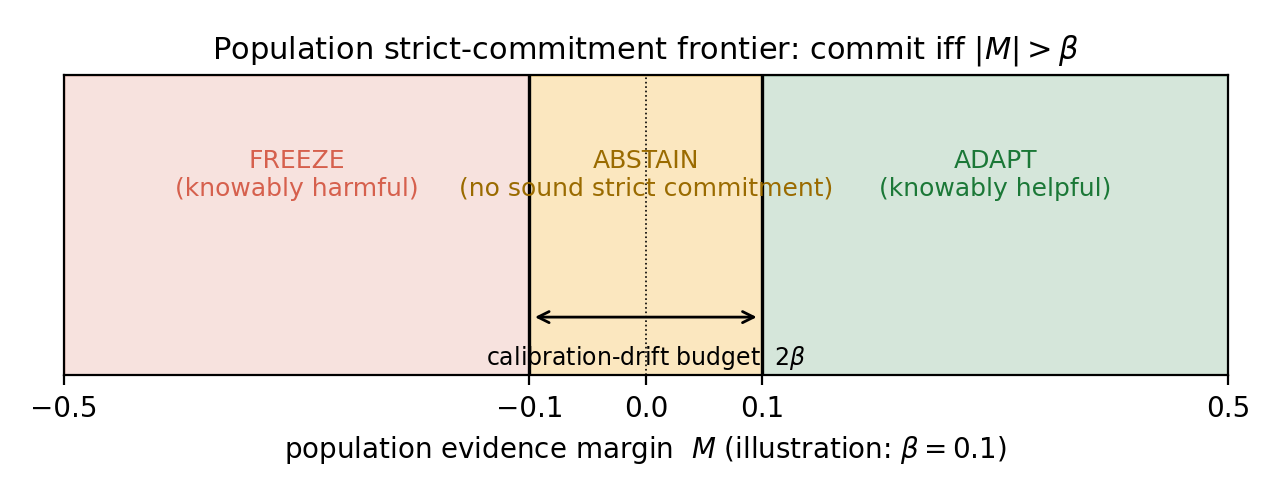
\includegraphics[width=0.95\linewidth]{figures/fig_frontier_schematic.png}
\caption{\textbf{Population strict-commitment frontier.} The population rule supports adapt or
freeze outside the drift band and abstains inside it. At the boundary, zero-benefit ambiguity rules
out a uniformly sound strict action; opposite nonzero signs are claimed only in the interior. KGA
uses the separate finite-sample interval rule in Fig.~\ref{fig:certificate}.}
\label{fig:frontier}
\end{figure}

\subsection{Formal Setup}
% Shared K-Bound theory setup (main text + appendix).
% Included by kbound_short.tex and main_theory_5.tex.

\noindent
Source law $P_S(X,Y)$ supplies labels at train/validation; target law $P_T(X,Y)$ exposes only
$P_T(X)$ at deployment. Fix loss $\ell$, frozen predictor $f_0$, candidate $f_a$, and target
measure $\mu_T$ on inputs. Write target risk $R_T(f)=\E_{P_T}[\ell(f(X),Y)]$ and the
\emph{adaptation benefit}
\[
\Delta \;:=\; R_T(f_0)-R_T(f_a)\qquad(\Delta>0\ \Leftrightarrow\ \text{adapting helps}).
\]
The \emph{disagreement region} $D:=\{x:f_0(x)\neq f_a(x)\}$ is observable from $(f_0,f_a)$.

\begin{assumption}[Deployment setup]\label{ass:deploy}
Unless stated otherwise: binary label $Y\in\{0,1\}$, $0/1$ loss $\ell$, and
$\mu_T(D)>0$. Fix a source-calibrated score $s:\mathcal{X}\to[0,1]$ estimating the candidate's
\emph{pointwise correctness} (e.g.\ a Platt-scaled confidence that $f_a$ is right at $x$), and write
the target pointwise correctness $\eta_a(x):=\Pr_T\!\bigl(f_a(X){=}Y\mid X{=}x\bigr)$ on $D$, so that
$\E_{\mu_T}[\eta_a\mid D]=\bar a$. Define the \emph{observable margin}
\[
M \;:=\; \E_{\mu_T}[s(X)\mid D]-\tfrac12,
\]
the \emph{calibration drift} (unobserved at deploy)
\[
\gamma \;:=\; \E_{\mu_T}[\eta_a(X)-s(X)\mid D],
\]
and label-free evidence $Z=\phi(X_{1:m},f_0,f_a)$ for any measurable
$\phi$ using only unlabeled batches and model outputs (entropy, confidence, drift,
disagreement, update norms). A \emph{label-free rule} is any measurable map
$g:\mathcal{Z}\to\{\textsc{adapt},\textsc{freeze},\textsc{abstain}\}$ that does not use target
labels on the deployment batch.
\end{assumption}

\begin{definition}[Risk alignment]\label{def:risk-align}
Evidence $Z$ is \emph{risk-aligned on a class $\mathcal{P}$} if no two laws
$P_T^1,P_T^2\in\mathcal{P}$ with $\sign\Delta_1\neq\sign\Delta_2$ satisfy
$\Law(Z\mid P_T^1)=\Law(Z\mid P_T^2)$.
\end{definition}

\begin{definition}[Regimes]\label{def:regimes}
At evidence $z$: \emph{knowably helpful} if the population frontier certifies $\Delta>0$
(\textsc{adapt}); \emph{knowably harmful} if it certifies $\Delta<0$ (\textsc{freeze});
\emph{unknowable} if the same $Z$-law is compatible with both signs (\textsc{abstain}).
\end{definition}

\begin{remark}[Four quantities]\label{rem:four-quantities}
Do not confuse $M$ (observable margin, deploy-time), $\gamma$ (realized drift, latent),
$\beta$ (declared bound $|\gamma|\le\beta$ on the deployment class), and $\varepsilon$
(finite-sample radius from held-out residuals). The radius $\varepsilon$ operationalizes
coverage; it is \emph{not} an estimate of $\beta$.
\begin{center}\footnotesize
\begin{tabular}{@{}lp{0.28\linewidth}lp{0.24\linewidth}@{}}
\toprule
Symbol & Meaning & At deploy? & Role \\
\midrule
$M$ & observable evidence margin & yes & evidence toward adapt/freeze \\
$\gamma$ & realized calibration drift & no & can reverse the benefit sign \\
$\beta$ & declared bound on $|\gamma|$ & externally supplied & population frontier \\
$\varepsilon$ & residual quantile radius & estimated pre-deploy & finite-sample certificate \\
\bottomrule
\end{tabular}
\end{center}
\end{remark}

\begin{center}\fbox{\parbox{0.95\linewidth}{\small
\textbf{What ``label-free'' means.} No target/test labels at deploy; labeled source and
held-out validation may calibrate $\widehat\Delta$ and $\varepsilon$. Evidence $Z$ uses only
unlabeled batches, predictions, entropy, drift, and update statistics. The method is
\textbf{target-label-free}, not label-free of all supervision: labels may be used only in the
source/validation calibration split, never in the deployment batch or held-out test decision.}}
\end{center}

\begin{center}\fbox{\parbox{0.95\linewidth}{\small
\textbf{K-Bound in one sentence.} The true adaptation-benefit sign is recoverable only when
label-free evidence exceeds the uncertainty created by calibration drift; otherwise the correct
action is abstention.}}
\end{center}

For a supplied drift budget $\beta\ge0$, the \emph{declared deployment class} is
\[
\mathcal{C}_\beta \;:=\; \bigl\{P_T:\ |\gamma(P_T)|\le\beta\bigr\}.
\]
Identifiability statements below are \emph{over $\mathcal{C}_\beta$}, not over arbitrary shifts.


\section{Theory}\label{sec:theory}
\subsection{Roadmap}
The theoretical spine has three layers, and they carry unequal weight. First, the risk difference
reduces to the region where the frozen and candidate predictions disagree, and the disagreement-region
accuracy splits into an observable margin $M$ and a residual $\gamma$; this layer is definitional
bookkeeping (Remark~\ref{rem:gamma-residual}) and we do not present it as a result. Second---and this
is the layer with mathematical content---matched label-free evidence can support incompatible nonzero
benefit signs inside the declared band, which establishes an abstention requirement that no estimator
can engineer away, and the same construction makes label-free auditing of the band itself vacuous.
Third, combining the two gives the population frontier, while a calibrated interval around
$\widehat\Delta$ yields the separate finite-sample decision rule.

% Core load-bearing theory for the short-paper main text (with proofs).

\subsection{Benefit Reduction and Matched-Evidence Impossibility}

The first result connects the decision target to the three population symbols. Agreement outside
$D$ contributes no risk difference. Binary complementarity on $D$ then makes the sign of benefit
depend only on $M+\gamma$.

\begin{lemma}[Disagreement-region reduction]\label{lem:reduction}
Under Assumption~\ref{ass:deploy}, with $\bar a:=\Pr_T(f_a{=}Y\mid D)$,
\begin{align*}
\Delta &= 2\,\mu_T(D)\bigl(\bar a-\tfrac12\bigr),\\
\sign\Delta &= \sign(\bar a-\tfrac12)=\sign(M+\gamma).
\end{align*}
The identity $\sign\Delta=\sign(M+\gamma)$ holds for \emph{every} target law; it does not
assume $|\gamma|\le\beta$.
\end{lemma}
\begin{proof}
Outside $D$, the two predictors agree and incur the same $0/1$ loss. On $D$, exactly one is
correct. The adapted and frozen accuracies conditional on $D$ are therefore $\bar a$ and
$1-\bar a$. Hence $\Delta=2\mu_T(D)(\bar a-\tfrac12)$. The definitions of $M$ and $\gamma$ give
\begin{align*}
M+\gamma
&=\Bigl(\E_{\mu_T\mid D}[s]-\tfrac12\Bigr)
  +\E_{\mu_T\mid D}[\eta_a-s]\\
&=\E_{\mu_T\mid D}[\eta_a]-\tfrac12
 =\bar a-\tfrac12.
\end{align*}
Because $\mu_T(D)>0$, the three quantities have the same sign.
\end{proof}

The reduction tells us which hidden quantity controls the sign. The harder question is
identification. Can two target worlds agree on every permitted observation while assigning
opposite signs to $\Delta$? Inside the declared band, the answer is yes.

\begin{theorem}[Interior matched-evidence impossibility]\label{lem:nonid}
Fix $\beta>0$. For any feasible margin $M\in[-\tfrac12,\tfrac12]$ with $|M|<\beta$, there exist
$P_T^+,P_T^-\in\mathcal{C}_\beta$ with the following properties:
\begin{gather*}
  \Law(\widetilde Z\mid P_T^+)=\Law(\widetilde Z\mid P_T^-),\\
  M(P_T^+)=M(P_T^-)=M,\\
  \sign\Delta_+=-\sign\Delta_-\ne0,
\end{gather*}
where $\widetilde Z=(Z,M)$. If $\beta=0$, then $\mathcal C_0$ forces $\gamma=0$ and
$\sign\Delta=\sign M$; matched-evidence ambiguity therefore requires $\beta>0$.
\end{theorem}
\begin{proof}
Choose $0<\delta<\min\{\beta-|M|,\tfrac12\}$. For
$\theta\in\{+1,-1\}$, apply Lemma~\ref{lem:fibre} with the constant correctness kernel
\[
  \eta_\theta(x)=\tfrac12+\theta\delta,\qquad x\in D,
\]
and use the same fixed label kernel outside $D$. Denote the resulting target law by
$P_T^\theta$. The input marginal, predictors, score, and source law are fixed, so $M$ is the
same under $P_T^+$ and $P_T^-$. Lemma~\ref{lem:fibre} also gives the same law of $Z$ in the two
worlds. Consequently,
$\Law(\widetilde Z\mid P_T^+)=\Law(\widetilde Z\mid P_T^-)$ for
$\widetilde Z=(Z,M)$.

It remains to verify class membership and the benefit signs. Under $P_T^\theta$,
$\bar a_\theta=\tfrac12+\theta\delta$ and
\[
  \gamma_\theta=\theta\delta-M,
  \qquad
  |\gamma_\theta|\le\delta+|M|<\beta.
\]
Thus both laws belong to $\mathcal C_\beta$. Lemma~\ref{lem:reduction} yields
$\Delta_\theta=2\mu_T(D)\theta\delta$. The two benefits are nonzero and have opposite signs.
\end{proof}
\noindent The two evidence laws coincide exactly because only the label kernel on $D$ changes.
This is not a rate-based Le Cam argument. Their total-variation distance is zero, so the conclusion
is exact non-identifiability rather than a lower bound that varies with separation.

Randomization cannot resolve two worlds that induce exactly the same evidence law. A controller
that limits both directional errors must instead leave most of its probability on ABSTAIN.

\begin{corollary}[Matched-evidence abstention lower bound]\label{cor:matched-abstain}
Fix $\alpha\in(0,\tfrac12)$ and the shared evidence law from Theorem~\ref{lem:nonid}. Let $g$ be
any possibly randomized label-free rule. If, in every admissible world,
\begin{align*}
  \Pr[g=\adapt,\Delta\le0]&\le\alpha,\\
  \Pr[g=\freeze,\Delta\ge0]&\le\alpha,
\end{align*}
then $\Pr[g=\abstain]\ge1-2\alpha$.
\end{corollary}
\begin{proof}
The rule has the same action probabilities in both worlds. Its ADAPT probability is at most
$\alpha$ in the negative world. Its FREEZE probability is at most $\alpha$ in the positive world.
The three action probabilities sum to one.
\end{proof}

\subsection{Boundary Case}

The interior construction gives opposite nonzero signs. The boundary needs a separate argument:
one evidence-compatible world with zero benefit is already enough to defeat a uniform strict claim.

\begin{proposition}[Boundary case and closed-band abstention]\label{prop:closed-band}
Fix $\alpha\in(0,\tfrac12)$. Under Definition~\ref{def:strict-sound}, abstention is the pointwise
maximal sound action throughout $|M|\le\beta$. Any label-free rule that controls both marginal
directional errors at level $\alpha$ must abstain there with probability at least $1-2\alpha$.
Opposite nonzero benefit signs are asserted only when $|M|<\beta$.
\end{proposition}
\begin{proof}
For $|M|<\beta$, apply Theorem~\ref{lem:nonid} and
Corollary~\ref{cor:matched-abstain}.

Now suppose $|M|=\beta>0$. The declared class contains a zero-benefit world with $\gamma=-M$ and
a strict-benefit world with $\gamma=0$. These worlds have the same augmented-evidence law. In the
zero-benefit world, both directional error events occur whenever the rule commits. Dual error
control therefore gives $\Pr[\adapt]\le\alpha$ and $\Pr[\freeze]\le\alpha$. It follows that
$\Pr[\abstain]\ge1-2\alpha$, and neither strict action is uniformly sound.

Finally, if $M=\beta=0$, then $\mathcal C_0$ forces $\gamma=0$ and $\Delta\equiv0$. The same
conclusion follows directly.
\end{proof}
\noindent This convention is stricter than task regret. When $\Delta=0$, adapt and freeze are
risk-equivalent, but neither certifies a strict sign.

\subsection{Exact Strict-Commitment Frontier}

We can now answer the population question completely. The theorem separates four jobs: reduction,
sufficiency outside the band, necessity inside the band, and maximality of the resulting rule.

\begin{theorem}[Exact strict-commitment frontier]\label{thm:headline}\label{thm:frontier}
Under Assumption~\ref{ass:deploy}, fix $(\mu_T,P_S,f_0,f_a,s)$ so that $M$ is determined. Let
$\beta\ge0$. Necessity and maximality use the full, rich class $\mathcal C_\beta$. In particular,
that class contains the evidence-identical kernels from Theorem~\ref{lem:nonid} and the zero-benefit
boundary law. For a narrower subclass not closed under these constructions, only sufficiency
follows without an additional richness assumption.
\begin{enumerate}
\item[\textnormal{(i)}] \textbf{Reduction.} For every $P_T$, $\sign\Delta=\sign(M+\gamma)$
(Lemma~\ref{lem:reduction}).
\item[\textnormal{(ii)}] \textbf{Sufficiency.} If $|M|>\beta$ and $P_T\in\mathcal{C}_\beta$, then
$\sign\Delta=\sign M$.
\item[\textnormal{(iii)}] \textbf{Necessity.} If $|M|<\beta$, two laws in $\mathcal C_\beta$ have
the same augmented-evidence law and opposite nonzero benefit signs. If $|M|=\beta>0$, the
admissible residual $\gamma=-\sign(M)\beta$ gives $\Delta=0$. If $M=\beta=0$, then
$\Delta\equiv0$ throughout $\mathcal C_0$. Thus $|M|\le\beta$ supports no uniform strict direction.
\item[\textnormal{(iv)}] \textbf{Strict-commitment iff.} At the fixed augmented-evidence law, a
strict action is uniformly directionally sound if and only if $|M|>\beta$. On the closed band,
abstention is the pointwise maximal sound action in the sense of
Definition~\ref{def:strict-sound}.
\end{enumerate}
The population rule $M>\beta\Rightarrow\adapt$, $M<-\beta\Rightarrow\freeze$,
$|M|\le\beta\Rightarrow\abstain$ is the pointwise maximal sound certificate on
$\mathcal{C}_\beta$.
\end{theorem}
\begin{proof}
Part~(i) is Lemma~\ref{lem:reduction}. For~(ii), suppose $M>\beta$ and
$|\gamma|\le\beta$. Then $M+\gamma>0$, so Lemma~\ref{lem:reduction} gives $\Delta>0$. The negative
case is symmetric.

For~(iii), Theorem~\ref{lem:nonid} supplies opposite nonzero signs when $|M|<\beta$. At
$|M|=\beta>0$, the boundary law with $\gamma=-\sign(M)\beta$ has zero benefit. When
$M=\beta=0$, every law in $\mathcal C_0$ has zero benefit. These cases preclude a uniform strict
direction throughout the closed band.

Part~(iv) combines (ii), (iii), and Proposition~\ref{prop:closed-band}. Sufficiency gives the unique
sound strict direction outside the band. The impossibility and boundary results rule out both
strict directions on the band.
\end{proof}
\noindent Outside the band, the permitted residual is too small to reverse the visible direction
$M$. Inside the band, the same evidence is compatible with a failed strict claim. Abstention is
therefore part of the identified answer, not a defect of the decision rule.

\noindent The same frontier is visible from the identified benefit set. Let $d=\mu_T(D)>0$. With
the observables fixed, the full declared class gives
\[
 \Delta(\mathcal C_\beta)
 =2d\left[\max\{-\tfrac12,M-\beta\},
          \min\{\tfrac12,M+\beta\}\right].
\]
The interval inside brackets is
$[-\tfrac12,\tfrac12]\cap[M-\beta,M+\beta]$. The first set enforces
$\bar a\in[0,1]$; the second enforces $|\bar a-\tfrac12-M|\le\beta$. Every point in their
intersection is attained by a constant correctness kernel on $D$. A strict direction is available
exactly when the entire benefit interval lies above or below zero.


\subsection{How the Results Fit Together, and Which Steps Are Substantive}
\begin{center}\small
\textbf{Thm.~\ref{lem:nonid}} (opposite-world label-kernel construction; $\TV=0$)
$\rightarrow$ \textbf{Cor.~\ref{cor:matched-abstain}} (abstention forced at rate $\ge1-2\alpha$)
$\rightarrow$ \textbf{Aud-A} (label-free budget audits are vacuous) \\[3pt]
{\itshape the row above is the content; the row below is bookkeeping and an assumption} \\[3pt]
disagreement-region reduction and the residual definition $\gamma:=\bar a-\tfrac12-M$
$\rightarrow$ identity $\sign\Delta=\sign(M+\gamma)$
$\rightarrow$ \textbf{Thm.~\ref{thm:headline}} (interval arithmetic $+$ the construction above) \\[3pt]
assumed coverage $\Pr[|\widehat\Delta-\Delta|\le\varepsilon]\ge1-\alpha$
$\rightarrow$ \textbf{Thm.~\ref{thm:certificate}} (three-line implication)
\end{center}
\noindent We separate the two rows deliberately. Theorem~\ref{thm:certificate} is an implication
from an assumed premise, and the premise---not the theorem---is where the difficulty lives;
\S\ref{sec:fa-identity} shows that on our stress grids the premise is supplied by a calibration
that makes the conclusion arithmetically unavoidable. Theorem~\ref{thm:headline}'s sufficiency
clause is likewise an inequality on an interval we defined. What cannot be obtained by definition
is the construction in Theorem~\ref{lem:nonid} and its audit corollary, and that is where we ask
the reader to look.

\subsection{Extensions and Deferred Results}
Additional minimax, anytime-valid, multicandidate, and one-bit results are retained in the long
manuscript (\texttt{kbound.tex}) and are not used by the short-paper claims; the
auditability of the drift budget itself is stated in Appendix~\ref{app:audit-short},
with proofs in the long manuscript. The saved iWildCam
streaming script computes its betting increments from frozen and adapted window accuracies, which
require target labels. We therefore retain that run only as a label-informed offline stress
diagnostic (on the native $35{,}360$-image iWildCam test stream, continual TENT collapses to a
cumulative macro-F1 of $0.02$ versus $0.26$ frozen, with predictions degenerating to a handful of
classes); it is not a label-free KGA deployment result and no streaming empirical claim is made
in this paper.

\subsection{Claim Scope}
The population theorem is conditional on the declared class $\mathcal C_\beta$, and the finite-sample guarantee is conditional on valid interval coverage. The theorem controls the marginal probabilities $\Pr(\textsc{adapt},\Delta\le0)$ and $\Pr(\textsc{freeze},\Delta\ge0)$; it does not automatically control the conditional error among committed actions. The framework does not claim that $\beta$ is identifiable from unlabeled deployment data, that the empirical radius $\varepsilon$ estimates $\beta$, or that calibration coverage transfers to arbitrary unseen domains without an assumption or correction.

\section{KGA Method}\label{sec:method}
\subsection{System Overview}
\textsc{KGA} is the paper's practical finite-sample method---a decision wrapper around a fixed
adapter, not a new adaptation objective and not a numerical implementation of the population
$|M|>\beta$ rule. The wrapper is \emph{adapter-interface agnostic}: it requires only that a
candidate can be proposed, evaluated on the batch, and rolled back. Its calibration is
\emph{adapter-specific}: the benefit model and radius are refit per dataset and per candidate
adapter, and cross-adapter transfer of a fitted calibration is disallowed because it violates the
false-adapt bound (Table~\ref{tab:abl-transfer}). We fit the
benefit estimator and its radius \emph{out of fold}, so the data used to fit $\widehat\Delta$ and
the data used to calibrate its residual are disjoint for every point.
On the per-cell stress grids (CIFAR-10-C and the synthetic grids), for each cell $i$ a gradient-boosted
$\widehat\Delta_{-i}$ is trained on the other $N{-}1$ cells and evaluated on cell $i$. The radius
$\varepsilon$ is then an upper empirical quantile of the leave-one-out residuals
$\{|\widehat\Delta_{-i}(Z_i)-\Delta_i|\}_{i=1}^{N}$---leave-one-condition-out cross-fitted empirical
residual calibration, so no
cell's residual uses an estimator that saw it. On the natural-shift protocols (Camelyon17, iWildCam,
Office-Home) the split is across domains: $\widehat\Delta$ and $\varepsilon$ are fit once on a dev
split and the untouched held-out target-domain conditions are scored a single time. At deploy we
extract $Z$ from an unlabeled batch and return adapt, freeze, or abstain (Algorithm~\ref{alg:kga}).
Labels enter only through the calibration split; the deployment batch and held-out test scorer never
use target labels for the adapter, $\varepsilon$, evidence, or rule selection. The coverage
guarantee is split-dependent. Every radius in this paper is the exact rank statistic
$\varepsilon=\rho_{(k)}$, $k=\lceil(n_{\mathrm{cal}}{+}1)(1-\alpha)\rceil$, unclamped, with
$\varepsilon=+\infty$ (hence \textsc{abstain}) when $k>n_{\mathrm{cal}}$, and with the scored cell
excluded from its own pool
(declared once in \S\ref{sec:exp-setup}); archived benchmark JSONs generated under the earlier
interpolated empirical quantile have been regenerated under this rule, and the regenerated value is
what is printed.
Under exchangeability and a clean split, this rank statistic supports finite-sample marginal
coverage. On the per-cell grids the pool is the leave-one-out residual vector rather than a clean
split, so what the grids demonstrate is \emph{calibration-set} coverage close to nominal (realized
$0.898$ at nominal $0.90$, $\alpha{=}0.10$)---and, as \S\ref{sec:fa-identity} makes explicit, that
realized figure is a deterministic function of $n$ under in-sample rank calibration, not a
measurement. This is the standard jackknife radius, which is distribution-free only
asymptotically under estimator stability; its formal finite-sample counterpart is the jackknife$+$
of Barber et al.\ (2021) at level $1-2\alpha$, which we note but do not implement. The decision
rule's false-adapt guarantee is stated under the coverage hypothesis (\S\ref{sec:method}), which the
empirical coverage approximately meets. This construction sits in a known landscape: weighted conformal corrects
coverage under known covariate shift~\cite{tibshirani2019conformal}, adaptive conformal tracks
coverage online~\cite{gibbs2021adaptive}, and beyond exchangeability the coverage gap is bounded by
the total-variation drift of the calibration pairs~\cite{barber2023beyond}, which is conceptually
related to but mathematically distinct from our disagreement-region calibration budget $\beta$. The certificate's marginal false-adapt control is risk
control in the RCPS/Learn-then-Test lineage~\cite{bates2021rcps,angelopoulos2025ltt}, specialized
to the adapt/freeze/abstain loss; PAC prediction sets give set-valued analogues under covariate
shift~\cite{park2022pac}.

\subsection{Evidence Map and Benefit Estimator}
The evidence map uses only unlabeled batches and model outputs, and is instantiated as two
label-free panels matched to the two calibration regimes below. On the controlled stress grids
(CIFAR-10-C, ImageNet-C, PACS) the base panel is an $11$-dimensional vector computed from the
frozen softmax $p_0$ and the adapted softmax $p_a$ on the adaptation batch: the mean predictive
entropy and mean confidence of $f_0$ and of $f_a$; the normalized marginal (predicted-class)
entropy of each; the entropy and marginal-balance drops between them; the fraction of adapted
predictions above confidence $0.9$ (a collapse indicator); the $\mathrm{KL}$ divergence between
the adapted and frozen predicted-class marginals; and the $\ell_2$ norm of the adapter's
parameter update. On the natural-shift protocols (Camelyon17, iWildCam, Office-Home, RxRx1) a
$16$-dimensional panel adds distribution- and disagreement-oriented statistics computed from the
frozen logits: entropy and confidence quantiles; the frozen/adapted prediction-disagreement rate;
the entropy gap; a free-energy source$\to$target shift; a batch-vs-running BatchNorm-statistic
$\mathrm{KL}$; an ATC-style threshold-accuracy estimate (its threshold fixed on \emph{source}
labels only, never target labels); and a source$\to$target confidence drop. The source-calibrated
correctness score $s$ of \S\ref{sec:theory} is operationalized by the adapted-confidence and
ATC-style features. \textsc{KGA} does not explicitly estimate the theoretical margin $M$; it learns the benefit $\widehat\Delta=h_\theta(Z)$ directly from the full evidence vector $Z$.

The benefit model predicts $\widehat\Delta=h_\theta(Z)$ from labeled development conditions;
$h_\theta$ is a gradient-boosted regression tree (scikit-learn
\texttt{GradientBoostingRegressor}, squared error, $250$ trees, depth $2$, learning rate $0.05$,
subsample $0.8$, seed $0$), refit \emph{per dataset and per candidate adapter} rather than shared,
so the estimator itself implies no cross-dataset transfer.
The complete schema for both panels---exact per-feature formulas and families---is given in
Appendix~\ref{app:evidence-schema} (Tables~\ref{tab:schema-base} and~\ref{tab:schema-rich}), with
per-adapter update hyperparameters in Table~\ref{tab:adapter-hparams}.

\begin{table}[t]\centering\scriptsize
\caption{Label-free evidence \emph{actually computed} by KGA. The $11$-dim base panel drives the
stress grids; the natural-shift protocols use a $16$-dim panel that adds the rows marked
\emph{(nat.)}. Exact formulas and per-track subsets are in the configuration files.}
\label{tab:evidence-map}
\begin{tabular}{@{}p{0.27\linewidth}p{0.63\linewidth}@{}}
\toprule
Family & Statistics \\
\midrule
Frozen output $Z_0$ & mean entropy, mean confidence, normalized marginal-class entropy; entropy/confidence quantiles \emph{(nat.)} \\
Adapted output $Z_a$ & mean entropy, mean confidence, normalized marginal entropy, frac.\ confidence $>0.9$ \\
Change $Z_{\rm change}$ & entropy drop, marginal-balance drop, entropy gap \\
Disagreement & frozen/adapted prediction-disagreement rate \emph{(nat.)} \\
Distribution drift & adapted-vs-frozen marginal $\mathrm{KL}$; free-energy shift, BN-statistic $\mathrm{KL}$, ATC/confidence drop \emph{(nat.)} \\
Update behavior & $\ell_2$ norm of the adapter parameter update \\
\bottomrule
\end{tabular}
\end{table}

\subsection{Out-of-Fold Uncertainty Calibration}
For calibration condition $i$, an estimator that did not train on $i$ produces $\widehat\Delta_{-i}(Z_i)$ and residual
\[
r_i=|\widehat\Delta_{-i}(Z_i)-\Delta_i|.
\]
The radius is a pre-specified upper residual quantile. On clean development/test splits, ordinary split conformal provides finite-sample marginal coverage under exchangeability. On stress grids, the reported radius uses leave-one-condition-out cross-fitted empirical residual calibration; its observed coverage does not imply the same finite-sample guarantee as split conformal, and jackknife+ is not claimed. We therefore report the calibration design and guarantee level separately for each track.

\begin{algorithm}[t]
\caption{\textsc{KGA}: Knowability-Guided Adaptation}
\label{alg:kga}
\begin{algorithmic}[1]
\Require Frozen $f_0$; adapter $\mathcal{A}$; batch $X_{1:m}$; $\widehat\Delta$, $\varepsilon$, $\alpha$
\Ensure Decision $g\in\{\textsc{adapt},\textsc{freeze},\textsc{abstain}\}$
\State $f_a \leftarrow \mathcal{A}(f_0, X_{1:m})$
\State $Z \leftarrow \phi(X_{1:m}, f_0, f_a)$
\State $\widehat\Delta \leftarrow \widehat\Delta(Z)$;\;
  $L \leftarrow \widehat\Delta-\varepsilon$;\; $U \leftarrow \widehat\Delta+\varepsilon$
\If{$L>0$} \State $g\leftarrow\textsc{adapt}$
\ElsIf{$U<0$} \State $g\leftarrow\textsc{freeze}$
\Else \State $g\leftarrow\textsc{abstain}$
\EndIf
\State \Return $g$
\end{algorithmic}
\end{algorithm}

\begin{figure}[t]\centering

\includegraphics[width=0.95\columnwidth]{figures/fig_certificate.png}
\caption{\textbf{The certificate rule in one picture.} \textsc{KGA} estimates the label-free benefit
$\widehat\Delta(Z)$ and forms an interval $\widehat\Delta\pm\varepsilon$: if the interval is entirely
positive it adapts, if entirely negative it freezes, and otherwise it abstains. The vertical axis here
uses true benefit only for offline audit; deployment decisions use only unlabeled evidence and the
pre-calibrated radius.}
\label{fig:certificate}
\end{figure}

On the good event $|\widehat\Delta-\Delta|\le\varepsilon$, committing adapt only when
$L>0$ implies $\Delta>0$ (Theorem~\ref{thm:certificate}). The implication requires measurable
marginal coverage; exchangeability or shift correction is used to justify coverage, while risk
alignment is relevant to the population interpretation and estimator transfer. No target labels are
used at deployment.

\subsection{Population Frontier versus Empirical Certificate}
\textsc{KGA}'s commit boundary is not a swept hyperparameter, but the population frontier and the
empirical radius must be kept distinct. The \emph{population} frontier of
Theorem~\ref{thm:headline} says a strict action is uniformly sound over $\mathcal C_\beta$ iff the
population margin $|M|$ exceeds the declared budget $\beta$. The realized drift satisfies
$|\gamma|\le\beta$ but is unobserved. KGA instead learns $\widehat\Delta$ from $Z$ and uses a
finite-sample residual-coverage radius $\varepsilon$, fixed before target-test scoring. The radius
neither estimates nor substitutes for $\beta$; conditional on valid coverage it controls marginal
decision errors without requiring risk alignment. Confidence-thresholding (ATC) and
agreement-trend selection (AGL) fit a scalar against a labeled or held-out signal and
predict \emph{accuracy}. \textsc{KGA} instead certifies a strict benefit direction with a calibrated
interval and, unlike a committal thresholded estimator,
\textsc{abstains} where that interval crosses zero. This behavior is consistent with the structural region
studied by Theorem~\ref{lem:nonid}, though finite-sample abstentions may also reflect sampling
uncertainty, estimator inadequacy, or calibration conservatism. The impossibility construction, not a tuned cutoff, is what separates
\textsc{KGA} from ``estimate accuracy, then threshold.''


\subsection{Selecting and Auditing the Drift Budget}
The drift budget $\beta$ is part of the declared deployment class, not a target-test-tuned hyperparameter. It may be justified from historical domain calibration gaps, a documented domain assumption, or an explicit stress envelope. Sensitivity analysis should report how decisions change over a pre-specified range of budgets. A smaller $\beta$ asserts stronger calibration transfer and increases commitment; a larger $\beta$ widens the abstention region. When no credible upper bound is available, the population frontier does not provide a robust sign certificate. Reporting $\beta=0$ is then only a zero-drift plug-in analysis, not an assumption-free or conservative guarantee.
Appendix~\ref{app:audit-short} states exactly when a \emph{computed} $\widehat\beta$ can replace
the declared budget, and the limits of any such audit.

\subsection{Deployment Semantics and Failure-Safe Behavior}
The shadow-state workflow is: (1) checkpoint the active model; (2) propose adaptation on a temporary
copy; (3) evaluate frozen and candidate outputs; (4) extract $Z$; (5) compute
$\widehat\Delta\pm\varepsilon$; (6) commit or roll back; and (7) log the configuration, evidence,
interval, and action. Abstention applies to the adaptation update, not to prediction. \textsc{Adapt}
commits the candidate; \textsc{freeze} rolls it back; and \textsc{abstain} retains the frozen state
while recording that evidence was insufficient rather than certifiably harmful. The implementation
should automatically freeze or abstain when evidence is missing, the batch is too small, a checkpoint
or adapter configuration differs from calibration, the evidence lies outside calibration support,
numerical values are invalid, or no valid radius is available. In the reference implementation (\texttt{kbound\_pkg}), the gate is applied per batch
(\texttt{KGA.decide\_from\_batch}); on \textsc{abstain} or \textsc{freeze} the adaptation optimizer
scales the candidate update by $\texttt{abstain\_scale}{=}0$, i.e.\ the update is skipped and the
frozen state $f_0$ is served---this is the rollback mechanism. The failure-safe defaults instantiate
the diagnostics of Table~\ref{tab:failure-modes}: abstain when the batch is smaller than the
calibration batch size, when $Z$ lies outside calibration support, when a checkpoint or
adapter-configuration hash differs from the calibrated one, or when the radius or evidence is
missing or numerically invalid. In continual operation the last certified state replaces $f_0$ as
the fallback.

\subsection{Computational Cost}
KGA cannot avoid the cost of proposing an update because candidate adaptation includes forward and
backward computation before commitment. The controller's \emph{added} cost is measured by a
controller-only microbenchmark (Table~\ref{tab:cost}): evidence
extraction $0.074$\,ms and benefit-model evaluation $0.127$\,ms per decision ($0.20$\,ms total),
plus one model copy ($44.8$\,MB, ResNet-18/CIFAR) for rollback; the benefit model itself is
$195$\,KB. Candidate adaptation and inference are unchanged by KGA---$f_a$ is evaluated
regardless---and are expected to dominate end-to-end latency, but this microbenchmark does not
measure them: a complete end-to-end component profile (frozen inference, candidate adaptation and
inference, rollback time, total window latency) remains pending (App.~\ref{app:runtime}).

\begin{table}[t]\centering\footnotesize
\caption{KGA controller \emph{added} cost (ResNet-18/CIFAR; controller-only microbenchmark).
Candidate adaptation/inference are unchanged by KGA and are \emph{not} measured here; the
end-to-end component profile is pending (App.~\ref{app:runtime}).}
\label{tab:cost}
\begin{tabular}{lc}
\toprule
Component & Cost \\
\midrule
Evidence extraction (per batch) & $0.074$\,ms \\
Benefit-model evaluation (per decision) & $0.127$\,ms \\
\textbf{Controller added latency} & $\mathbf{0.20}$\,\textbf{ms} \\
Rollback model copy (memory) & $44.8$\,MB \\
Benefit model size & $195$\,KB \\
\bottomrule
\end{tabular}
\end{table}

\section{Experimental Setup}\label{sec:exp-setup}
\subsection{Research Questions}
The experiments address seven questions: \textbf{RQ1} whether the decision code implements the population frontier as specified (a wiring check on synthetic ground truth, \emph{not} a test of the frontier --- see \S\ref{sec:synthetic}); \textbf{RQ2} whether the interval controls marginal false adaptation \emph{where that is testable} --- wherever a rank radius is computed in-sample it makes $\mathrm{FA}_{\mathrm u}\le\alpha$ an arithmetic identity rather than a measurement (\S\ref{sec:fa-identity}), so RQ2 is really the question of how many \textsc{adapt} decisions a track makes under a leave-one-out radius and whether any of them is wrong; \textbf{RQ3} whether KGA assigns \textsc{adapt}, \textsc{freeze}, and \textsc{abstain} consistently with helpful, harmful, and low-margin conditions; \textbf{RQ4} whether it prevents damage on held-out natural shifts; \textbf{RQ5} whether it improves decision validity over simple and neighboring label-free gates; \textbf{RQ6} which evidence and calibration choices matter; and \textbf{RQ7} what computational overhead the controller adds.

\subsection{Datasets and Shift Taxonomy}
The evaluation separates controlled corruption/composition stress, large-scale corruption, natural institutional or geographic shifts, domain generalization, and low-margin diagnostic transfers. This taxonomy matters because mixed conditions test action discrimination, one-sided shifts test safe commitment, and low-margin transfers test abstention. The nine tracks draw on CIFAR-10-C~\cite{hendrycks2019cifar10c}, ImageNet~\cite{deng2009imagenet}, the WILDS Camelyon17, iWildCam, and RxRx1 shifts~\cite{koh2021wilds,bandi2019camelyon,taylor2019rxrx1}, Office-Home~\cite{venkateswara2017officehome}, PACS via DomainBed~\cite{gulrajani2021domainbed}, and CIFAR-10.1~\cite{recht2019cifar10}; models build on RobustBench checkpoints~\cite{croce2021robustbench} with PyTorch~\cite{paszke2019pytorch} and scikit-learn~\cite{pedregosa2011sklearn}.

\begin{table*}[t]\centering\scriptsize
\caption{Dataset roles in the evaluation. The expected regime is a hypothesis fixed by the protocol, not a conclusion inferred from the final score.}
\label{tab:dataset-taxonomy}
\begin{tabular}{@{}llll@{}}
\toprule
Track & Shift type & Candidate role & Evaluation purpose \\
\midrule
CIFAR-10-C stress & corruption/composition/update stress & Tent/EATA (SAR withheld) & mixed detectable decision benchmark \\
ImageNet-C noise & large-scale corruption & Tent/EATA/SAR & scale and candidate dependence \\
Camelyon17 & hospital/institution shift & EATA & helpful-dominated natural safety \\
iWildCam & geographic camera shift & Tent & harmful-dominated natural safety \\
Office-Home & visual domain/style shift & SAR & held-out domain safety \\
RxRx1 & experimental/laboratory shift & online adapter & harmful-dominated natural safety \\
PACS & domain generalization & fixed candidate & breadth and null behavior \\
ImageNet-R & rendition shift & candidate panel & weak-evidence diagnostic \\
CIFAR-10.1 & natural resampling & TTA candidates & low-margin transfer diagnostic \\
\bottomrule
\end{tabular}
\end{table*}

\subsection{Models, Adapters, and Leakage Control}
For every track, the source checkpoint, candidate adapter, update mode, learning rate, number of steps, batch construction, adapted parameter subset, and random seeds must be declared before held-out scoring. Adapter selection, evidence selection, benefit-model fitting, and residual calibration use development data only. All choices are frozen before the target test cells are scored once; target labels are opened afterward solely for offline audit. The calibration and scoring configuration is uniform across tracks except where noted in Table~\ref{tab:config-table}.

\paragraph{The quantile rule, declared once.}\label{par:quantile-rule}
Every radius reported in this paper is the \textbf{exact-rank} order statistic
\[
\varepsilon=\rho_{(k)},\qquad k=\big\lceil (n_{\mathrm{cal}}{+}1)(1-\alpha)\big\rceil,\qquad
\alpha=0.10,
\]
computed on the residual vector defined by the track's calibration unit
(Table~\ref{tab:config-table}). There is \textbf{no $\min\{n_{\mathrm{cal}},\cdot\}$ clamp}. When
$k>n_{\mathrm{cal}}$ the rule is \emph{infeasible} --- no finite radius attains $1-\alpha$, because
the best attainable coverage is $n_{\mathrm{cal}}/(n_{\mathrm{cal}}{+}1)$ --- and the released
library (\texttt{kga.certificate.split\_conformal\_rank\_radius}) returns
$\varepsilon=+\infty$ with a warning, which forces \textsc{abstain}. At $\alpha=0.10$ this makes
$n_{\mathrm{cal}}\ge\lceil1/\alpha\rceil-1=9$ the feasibility threshold. Earlier drafts of this
paper declared the \emph{clamped} variant $k=\min\{n_{\mathrm{cal}},\cdot\}$; that variant silently
returns the largest residual and attains only $n_{\mathrm{cal}}/(n_{\mathrm{cal}}{+}1)<1-\alpha$, so
it is not the rule we claim under. It survives in the library solely as an opt-in replay flag
(\texttt{on\_infeasible='clamp'}) for reproducing archived numbers, and we do not use it for any
number in this paper.

\emph{The clamp is never binding here, and we checked.} At every calibration size that occurs in
this paper, $k\le n_{\mathrm{cal}}$: $n{=}9\Rightarrow k{=}9$, $n{=}12\Rightarrow k{=}12$,
$n{=}18\Rightarrow k{=}18$, $n{=}27\Rightarrow k{=}26$, $n{=}135\Rightarrow k{=}123$,
$n{=}432\Rightarrow k{=}390$. So clamped and unclamped agree on every printed value, and the
distinction matters for what the paper \emph{claims}, not for what it prints. The one place the
threshold does bite is the leave-one-out-of-pool pool of size $n_{\mathrm{cal}}-1$
(next paragraph): at $n_{\mathrm{cal}}=9$ the leave-one-out pool has $8$ residuals and $k=9>8$, so
leave-one-out-of-pool is \emph{infeasible} on the $9$-condition Camelyon17 per-seed pools of
Table~\ref{tab:multiseed}; those are scored in-pool and their
$\mathrm{FA}_{\mathrm u}$ column is accordingly uninformative (\S\ref{sec:fa-identity}).

This is the only radius rule used anywhere in the paper; wherever an earlier
draft or an archived artifact reported the interpolated empirical quantile
\texttt{np.quantile}$(\rho,1-\alpha)$, the number has been regenerated under the rule above and the
regenerated value is the one printed. The two rules are not cosmetically different: on ImageNet-C SAR
they give pooled regret $0.0289$ (exact rank) versus $0.0122$ (interpolated), a factor of $2.4$, and
they differ in the number of \textsc{adapt} decisions by $13$ versus $61$ out of $135$. Adopting the
exact-rank rule uniformly also moves three other published rows relative to earlier drafts:
ImageNet-R $0.0112\to0.0151$, CIFAR-10.1 SAR $0.0045\to0.0057$, and Camelyon17 Table~\ref{tab:multiseed}
SAR $0.0410\to0.0425$; the CIFAR-10-C rows move in the fourth decimal only
($0.0015736\to0.0015852$ Tent, $0.0012676\to0.0012799$ EATA). We report the exact-rank value in every
case, including where it is the less favourable of the two.

\paragraph{The pool, declared once: leave-one-out-of-pool.}\label{par:loo-pool}
A radius computed from a pool that \emph{contains the residual of the cell being scored} is a
function of that cell's label, which is the label the $\mathrm{FA}_{\mathrm u}$ guarantee is about.
Every per-cell radius in this paper therefore excludes the scored index: cell $i$'s radius is
$\rho_{(k)}$ over the other $n_{\mathrm{cal}}-1$ residuals
(\texttt{kga.certificate.conformal\_radii\_loo}). On the split-calibrated natural-shift tracks the
question does not arise --- the calibration domains and the scored domains are disjoint by
construction. The correction is free on CIFAR-10-C and is not free on ImageNet-C: it changes
\textbf{$0$ of $9{,}504$} committed CIFAR-10-C decisions and leaves $\mathrm{FA}_{\mathrm u}=0$
throughout, while on ImageNet-C SAR it changes $2$ of $135$ decisions and moves the promoted
triple from $0.0264$ to $0.0289$ with $\mathrm{FA}_{\mathrm u}$ from $0$ to $1/135$
(\S\ref{sec:imagenetc}). We promote the leave-one-out value on both tracks.

\begin{table}[t]\centering\scriptsize
\caption{Per-track calibration and scoring configuration ($\alpha{=}0.10$ throughout; benefit
estimator family and calibration recipe are used across tracks, with parameters refit per dataset and candidate adapter, \S\ref{sec:method}). The radius rule is the same unclamped exact-rank order statistic
$\rho_{(k)}$, $k=\lceil(n{+}1)(1-\alpha)\rceil$ ($+\infty\Rightarrow\textsc{abstain}$ if $k>n$), in
every row---only the residual pool
differs. The two grid rows exclude the scored cell from its own pool
(\S\ref{par:loo-pool}); the split-calibrated rows do so by construction. Backbones: ResNet-18 (CIFAR), ResNet-50
(ImageNet-C); the natural-shift backbones follow the WILDS/DomainBed defaults per track.}
\label{tab:config-table}
\begin{tabular}{@{}p{0.24\linewidth}p{0.30\linewidth}p{0.34\linewidth}@{}}
\toprule
Track & Residual pool for $\rho_{(k)}$ & Test unit \\
\midrule
CIFAR-10-C stress & grid cell (leave-one-cell-out) & $5{\times}432$ cells \\
ImageNet-C & grid cell (leave-one-cell-out) & $27$ cells $\times\,5$ seeds \\
PACS (LODO) & source-domain cells & $18$ cells/target/seed; $3$ seeds \\
Camelyon17 & dev domains $\{0,1\}$, out-of-fold & test $\{2,3,4\}$ \\
iWildCam H v2 & calibration domain $\{0\}$, out-of-fold & held-out $\{1\}$ \\
Office-Home M v2 & calibration $\{0,1\}$, out-of-fold & target test $\{0,1\}$ \\
RxRx1 J & development $\{0,\ldots,4\}$, out-of-fold & test $\{5,\ldots,9\}$ \\
\bottomrule
\end{tabular}
\end{table}
Two caveats attach to the rule rather than to any track. First, on the stress grids the residual pool
is leave-one-\emph{cell}-out, i.e.\ a jackknife, not a clean split; it therefore carries empirical
rather than distribution-free coverage (\S\ref{sec:method}), and Algorithm~\ref{alg:calib-eval} labels
each branch accordingly. Second, wherever a radius is nonetheless computed from the same vector it is
used to test --- which in this paper is only the $n{=}9$ Camelyon17 per-seed pools of
Table~\ref{tab:multiseed}, where leave-one-out is infeasible --- $k$ equals $n$ exactly, so
$\varepsilon$ is the maximum residual, $\mathrm{FA}_{\mathrm u}$ is forced to $0$, and that column
carries no information; see \S\ref{sec:fa-identity}.
Exact per-adapter update settings (optimizer, steps, learning rate, and the mild/aggressive
operating points) are tabulated per track in Appendix~\ref{app:evidence-schema},
Table~\ref{tab:adapter-hparams}.

\subsection{Baselines}
We distinguish fixed policies (always-freeze and always-adapt), an offline per-condition oracle, simple label-free gates (confidence, entropy, drift/KL, and ATC-style), KGA without its radius, and neighboring methods or ports inspired by POEM and AETTA. Each comparison must state whether the baseline is an official implementation, a faithful reimplementation, or a protocol-matched port.

\subsection{Metrics and Statistical Testing}
The primary decision metrics are regret-to-oracle, marginal false-adapt $\mathrm{FA}_{\mathrm u}=\Pr(\textsc{adapt},\Delta\le0)$, conditional false-adapt $\mathrm{FA}_{\mathrm c}=\Pr(\Delta\le0\mid\textsc{adapt})$, adapt rate, action composition, and decision coverage $\Pr(\textsc{adapt or freeze})$. Accuracy or AUROC is reported as a task metric, not as the controller's objective. The theorem controls $\mathrm{FA}_{\mathrm u}$ under its assumptions; $\mathrm{FA}_{\mathrm c}$ is descriptive. Lower regret than both fixed policies is a secondary routing-utility check and does not establish interval coverage or risk alignment. Paired bootstrap confidence intervals, their resampling unit, and seed aggregation are declared per comparison family.

\paragraph{The multiplicity family, declared prospectively.}\label{par:multiplicity}
Earlier versions of this work declared the Holm family as ``the three beats-both candidates
(CIFAR-10-C Tent/EATA versus always-adapt; ImageNet-C SAR versus always-freeze), all of which
survive Holm at $0.05$'' --- that is, exactly the three comparisons that came out positive, named
after the results were known. That is not a multiplicity correction and we withdraw it. The
project's search history is public and large: across the committed campaign artifacts there are
$1{,}387$ recorded \texttt{beats\_both} determinations ($326$ of them true, a $23.5\%$ base rate)
over $70$ distinct scored result units and $69$ pre-registered protocol files, with directory names
(\texttt{win\_hunt\_v2}--\texttt{v5}, \texttt{win\_finder\_v*}, \texttt{hard\_dataset\_win\_loop\_v1})
that describe the search accurately. Most of those rows are exploratory development screens and do
not belong in an inferential family, but the paper previously published no arm inventory at all, so
a reader had no way to judge.

We therefore define the family \emph{prospectively} as follows. The confirmatory family is the set
of \textbf{pre-registered beats-both bars} --- one per (track, candidate) pair named in a
\texttt{research\_lock/} protocol before any number for that pair was computed --- evaluated once on
the declared test cells. Rows produced by development screens, superseded protocol versions, or
post hoc re-scorings are \emph{not} members of that family and are not eligible for promotion, no
matter how they come out. Appendix~\ref{app:arm-inventory} publishes the resulting protocol $\to$
arms $\to$ verdict inventory in full, including the arms that failed, and Holm is applied over that
inventory rather than over the winners. Readers who want the raw, uncorrected picture should read
the appendix table, not the three intervals in the main text.

\subsection{Defining ``mixed and detectable''}\label{sec:detectability}
Earlier versions of this work asserted that \textsc{KGA} beats both fixed policies ``whenever
helpful and harmful conditions are mixed and detectable'' without ever saying what \emph{detectable}
means. As written that claim was unfalsifiable: the regimes labelled detectable were exactly the
regimes where the win occurred. We replace it with an ex ante criterion, applied to every track
before its outcome is discussed.

\begin{definition}[Mixed, detectable]\label{def:detectable}
A track is \textbf{mixed} at threshold $p$ if its harmful base rate---the fraction of evaluation
cells with $\Delta\le0$---lies in $[p,1-p]$; we fix $p=0.10$. A mixed track is \textbf{detectable}
at level $\alpha$ if the cross-fitted certificate strictly commits (\textsc{adapt} or
\textsc{freeze}, i.e.\ $|\widehat\Delta|-\varepsilon>0$) on at least $25\%$ of its cells. Both
quantities are computable from the logged decisions without target labels beyond the offline audit,
and neither refers to the regret comparison.
\end{definition}

Applying Definition~\ref{def:detectable} to the nine tracks: CIFAR-10-C Tent (harmful $0.34$,
decision coverage $0.68$) and EATA ($0.27$, $0.63$) are mixed and detectable; ImageNet-C SAR
($0.156$, $26/135=0.19$) is mixed but sits \emph{below} the coverage bar and is therefore
\textbf{not} detectable by our own criterion despite producing a win --- we flag this rather than
move the bar; ImageNet-C Tent ($0.556$, $0/135$) is the most mixed track in the paper and is
decisively \emph{not} detectable; ImageNet-C EATA ($0.02$) and Camelyon17 ($0.00$--$0.11$ per
candidate) are not mixed; PACS is mixed (mean harmful base rate $0.278$) and passes the coverage bar
($0.815$) yet loses to always-adapt --- a clean counterexample to sufficiency; ImageNet-R is mixed on
only $3$ of $10$ backbones; RxRx1 and iWildCam are harmful-dominated one-sided tracks. Four tracks
meet the mixed bar: CIFAR-10-C Tent and EATA meet detectability and produce a point-estimate
beats-both (cluster-robust for Tent only, \S\ref{sec:cifar-stress}); PACS meets
detectability and \emph{loses} to always-adapt; ImageNet-C Tent fails detectability outright and
produces nothing. ImageNet-C SAR produces a point-estimate beats-both without meeting our coverage
bar, and without an interval to support it either. So the
criterion is neither necessary nor sufficient on our own data, and the correct statement is the weak
one: \emph{a routing win requires mixed conditions, but mixedness plus decisiveness does not deliver
one}. We say so rather than tune the thresholds until the sentence becomes true.

\subsection{Evidence-Status Policy}\label{sec:evidence-policy}
\textbf{Locked} results trace to raw cells/seeds and a frozen aggregate; \textbf{reconciled} results correct a prior interpretation using raw records; \textbf{provisional} summaries require canonical replay; and \textbf{diagnostic} runs are complete but deliberately not promoted. Only locked and reconciled rows support the empirical headline. Every evidence-tier cell in the result tables begins with one of these four labels; qualifiers (seed counts, lock type, known caveats) follow in parentheses.

\subsection{Hardware and Software}
Runs use Python~3.12, PyTorch~2.5.1, and scikit-learn for the benefit estimator. Accelerator and
checkpoint details are recorded per run manifest rather than pooled into one hardware claim:
CIFAR experiments used the saved ResNet-18 setup; the authoritative ImageNet-C result used
ResNet-50 on seeds~$0$--$4$. Hardware affects runtime but not the decision definitions or replayed metrics.

\section{Results}\label{sec:exp}
The results are organized by regime rather than by dataset prestige, and they are read as a safety evaluation. The primary result is that on the four one-sided natural tracks with locked held-out artifacts KGA is no-harm---the deployment guarantee an operator wants---while on the three remaining natural tracks it is a conservative null or a declared failure, which we report in the same table rather than in a footnote. Controlled mixed regimes then test action discrimination and selective coverage and supply the secondary beats-both mechanism confirmation, and low-margin transfers test whether the method declines unsupported claims. Accuracy and regret are reported as descriptive task metrics throughout, not as the controller's objective.

%% fig:regime-map (fig_phase_diagram.png) removed: its own caption conceded it was a conceptual
%% schematic with illustrative rather than measured axis coordinates, duplicating
%% Table~\ref{tab:regime-summary}. No \ref pointed at it.

\subsection{Synthetic illustration of the frontier (not a test of it)}\label{sec:synthetic}
Before the real-data tracks we \emph{illustrate} the population rule on synthetic ground truth, where
the observable margin $M$, the unobserved drift $\gamma\sim\mathrm{U}(-\beta,\beta)$, and hence the
true benefit sign $\sign\Delta=\sign(M+\gamma)$ are all controlled. We label this an illustration
rather than a validation, and we say plainly why, because the distinction was blurred in earlier
versions of this work.

\paragraph{Why this cannot falsify the frontier.} In the generator, the evidence $Z$ is four copies
of $M$ perturbed by Gaussian noise of scale $0.02$, and the benefit is $B=M+\gamma$. Any competent
regressor therefore recovers $\widehat\Delta\approx M$, which makes the residual
$|\widehat\Delta-\Delta|$ equal to $|\gamma|$ up to observation noise, so the conformal radius
converges to $q_{0.9}(|\mathrm U(-\beta,\beta)|)=0.9\beta$ \emph{by algebra}. The commit rule
$|\widehat\Delta|>\varepsilon$ is then $|M|>0.9\beta$: the frontier is not discovered, it is
substituted in. For the same reason the reported ``$90.0\%$ empirical coverage'' is not evidence of
anything --- \texttt{np.quantile} at level $0.9$ returns a value with exactly $90\%$ of the sample
below it for \emph{any} input, and we verified it is exactly $0.900$ at both $n{=}400$ and $n{=}220$.
The generator's own docstring states the mechanism. This experiment demonstrates that the
implementation computes what the theory says; it cannot come out negative and so it tests nothing.

\paragraph{What it shows.} With that caveat, the run is internally consistent
(Fig.~\ref{fig:frontier-measured}; $\alpha{=}0.10$): $\widehat\Delta$ tracks $\Delta$; the commit rate
moves from $6.5\%$ for $|M|<\beta$ to $96.7\%$ for $|M|>\beta$ and the committed sign is correct
$99.3\%$ of the time; and $\mathrm{FA}_{\mathrm u}\le0.014$ for every
$\beta\in\{0.05,\ldots,0.20\}$. Read it as a wiring check on the decision code, at the level of a
unit test.

\paragraph{The experiment that would test it, and why we have not run it.} A genuine test of the
population frontier requires $M$ computed from data rather than drawn, evidence that is not a noisy
copy of $M$, a $\gamma$ whose $0.9$-quantile is not $\beta$, and a held-out scoring set. The natural
design on our own tracks is a $\beta$ sweep on the CIFAR-10-C grid: take $M$ from the ATC-style
source-calibrated correctness score already in the rich evidence panel (\S\ref{sec:method}), declare
$\beta$ from historical dev-to-deployment calibration gaps rather than from the test residuals,
sweep $\beta\in\{0,0.02,0.05,0.10,0.20\}$, and run the population rule $M\gtrless\pm\beta$ against
the realized benefit signs on held-out cells. That experiment is not in this paper. Its absence is
the single largest gap in our evidence: as things stand, \textbf{the population theory has no contact
with any of the nine benchmark tracks}, and $\beta$ is never numerically supplied to \textsc{KGA} on
real data (the empirical decision uses $\widehat\Delta\pm\varepsilon$ throughout). We flag it as the
first item of future work, and note that a \emph{negative} result there would be more informative
than the present silence.

\begin{figure}[t]\centering
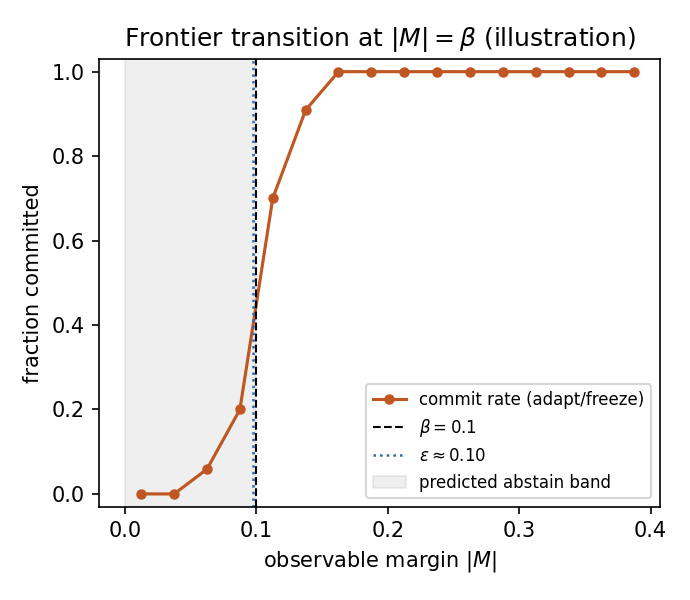
\includegraphics[width=0.86\columnwidth]{figures/fig_frontier_transition.png}
\caption{\textbf{Benefit-sign frontier, synthetic illustration} (archived cross-fitted rule). The
commit rate transitions sharply from abstention to adapt/freeze near $|M|{=}\beta$ and the calibrated
radius $\varepsilon$ (dotted) tracks $\beta$ --- both by construction, since the generator's residual
is exactly $\gamma$ and $q_{0.9}(|\gamma|)=0.9\beta$ (\S\ref{sec:synthetic}). This figure is a wiring
check, not a test. Companion panels---estimator recovery
and $\mathrm{FA}_{\mathrm u}\le\alpha$ across $\beta$---in
\texttt{fig\_frontier\_recovery.png}, \texttt{fig\_frontier\_fa\_coverage.png}.}
\label{fig:frontier-measured}
\end{figure}

\subsection{CIFAR-10-C stress grid (5 seeds)}\label{sec:cifar-stress}
\paragraph{What the grid is.} The \emph{stress} grid crosses corruption, severity,
batch size, composition, and update aggressiveness ($432$ conditions/method, ResNet-18;
pre-registered as Protocol~A; seeds $0$--$4$). Its exact composition is
$6\ \text{corruptions}\times2\ \text{severities}\times3\ \text{batch regimes}\times3\ \text{compositions}
\times2\ \text{aggressiveness levels}\times2\ \text{repeats}=432$. The six corruptions are
\texttt{contrast}, \texttt{defocus\_blur}, \texttt{fog}, \texttt{gaussian\_noise},
\texttt{jpeg\_compression}, and \texttt{pixelate}, at severities $\{1,5\}$ --- that is
\textbf{$6$ of the $15$ official CIFAR-10-C corruptions and $2$ of the $5$ severities}, selected by
the driver's \texttt{--quick} subset (\texttt{"quick": true} appears in every run manifest). Nine
corruptions are absent, including the rest of the noise family (\texttt{shot\_noise},
\texttt{impulse\_noise}), the weather corruptions (\texttt{snow}, \texttt{frost},
\texttt{brightness}), and \texttt{glass\_blur}, \texttt{motion\_blur}, \texttt{zoom\_blur},
\texttt{elastic\_transform}. Earlier versions of this work described the grid as covering ``the
official CIFAR-10-C corruptions''; that was wrong and is corrected here. Note also that the two
repeats \texttt{r0}/\texttt{r1} are exact design-point replicates and correlate at $0.948$ (adapt
gap) to $0.999$ (freeze gap), so the effective number of independent conditions is at most $216$,
not $432$.

\paragraph{Result.} Harmful base rates are $34\%$ (Tent) and
$27\%$ (EATA). The primary result is selective routing at $0\%$
false-adapt (Table~\ref{tab:decisive}). Among harmful cells \textsc{KGA} adapts $0$ and freezes them;
among helpful cells it adapts almost all; on marginal cells it abstains. This is the one track in
the paper where the false-adapt guarantee is exercised at power: $1{,}113$ (Tent) and $1{,}244$
(EATA) \textsc{adapt} decisions, none of them wrong, Clopper--Pearson $95\%$ upper bounds on
$\mathrm{FA}_{\mathrm c}$ of $0.0027$ and $0.0024$ (\S\ref{sec:fa-identity}).

\paragraph{The beats-both claim, separated by candidate.} Both candidates beat both fixed policies
on the point estimate. They do \emph{not} survive the same interval scrutiny, and we report them
separately rather than as one sentence. The $432$ conditions are not $432$ independent draws: the
design crosses $6$ corruptions with $2$ severities and duplicates every design point
(\texttt{r0}/\texttt{r1} correlate at $0.948$--$0.999$), so the honest resampling units are the
$216$ twin-pairs and, more conservatively, the $12$ corruption$\times$severity or $6$
corruption-family clusters. Table~\ref{tab:cifar-cluster} gives the paired-bootstrap gaps at all
four units.
\begin{itemize}
\item \textbf{Tent survives every unit.} The gap to always-adapt stays negative with the interval
excluding zero from $432$ cells down to $6$ corruption clusters ($[-0.00952,-0.00259]$), and so does
the gap to always-freeze. Clustering widens the intervals by $2.3\times$ (adapt side) and
$3.9\times$ (freeze side) --- a real cost, not a fatal one.
\item \textbf{EATA does not.} Its adapt-side gap loses the interval as soon as the corruption
structure is respected: $[-0.00483,+0.00043]$ at $12$ corruption$\times$severity clusters and
$[-0.00436,+0.00035]$ at $6$ corruption families, both containing zero. \textbf{We therefore claim
a CI-supported beats-both for Tent only.} For EATA the supportable statement is: a point-estimate
beats-both, CI-supported against always-freeze at every unit, and \emph{not} CI-supported against
always-adapt once corruption is treated as the cluster.
\end{itemize}
The per-corruption breakdown says the same thing at the level of the individual family. Tent is
worse than always-adapt on one of six corruptions (\texttt{gaussian\_noise}, adapt gap
$+0.00189$); EATA is worse on \emph{two} (\texttt{gaussian\_noise} $+0.00022$,
\texttt{jpeg\_compression} $+0.00292$). Six families is a small enough number that one or two
adverse ones is exactly what a cluster bootstrap should, and does, convert into an interval that
touches zero.\footnote{The design-based intervals we reported previously resample the
pre-registered mixing-ratio distribution of the stress-grid design (Protocol~A; the $11$-point
Pareto over harmful fraction, $N_{\mathrm{boot}}{=}5000$): Tent $+0.019\,[0.011,0.026]$ vs.\
always-adapt, $+0.080\,[0.052,0.107]$ vs.\ always-freeze; EATA $+0.015\,[0.009,0.021]$ and
$+0.075\,[0.049,0.100]$. Those intervals treat the mixing ratio as the only source of variation and
are not cluster-robust; where they disagree with Table~\ref{tab:cifar-cluster}, the cluster-robust
row is the one we claim on.}

\paragraph{Leave-one-corruption-out calibration.} The radius on this grid is calibrated
leave-one-\emph{cell}-out, so the calibration pool for a cell contains the other five severities and
repeats of the \emph{same} corruption. That is the most favourable partition available. Refitting
the whole pipeline leave-one-\emph{corruption}-out --- six folds, the estimator never sees the
corruption it is scored on --- degrades every intermediate quantity and the decision still holds
(bottom row of Table~\ref{tab:cifar-cluster}): residual MAE $0.00959\to0.03090$ ($3.2\times$),
$R^2$ $0.993\to0.895$, $\varepsilon$ $0.0213\to0.0988$ ($4.6\times$), adapt rate $51.5\%\to41.3\%$,
and \textsc{KGA} regret $0.00159\to0.00603$ ($3.8\times$) --- still below always-adapt's $0.00792$
and always-freeze's $0.12410$, at $\mathrm{FA}_{\mathrm u}=0$ under every partition. This is the
strongest single robustness result in the paper and it is a Tent result: we have not run the
corresponding refit for EATA.

\paragraph{The withheld SAR arm.} SAR on this grid is quarantined and we draw no comparative verdict
from it. The five-seed aggregate ($0.0015/0.0112/0.1286$) is dominated by seed $0$, whose harmful base
rate is $0.5278$ --- $5.8\times$ the mean of seeds $1$--$4$ ($0.0909$). On seeds $1$--$4$ alone
\textsc{KGA}'s regret ($0.0015990$) \emph{exceeds} always-adapt's ($0.0003099$) by $5.2\times$, and
$1$ of $5$ seeds beats both fixed policies --- seed $0$, the seed the quarantine exists for. The
adapt-gap bootstrap interval is entirely \emph{positive} (i.e.\ against \textsc{KGA}) at every
resampling unit we tried: $[+0.00101,+0.00158]$ over $432$ cells, $[+0.00003,+0.00298]$ over $12$
corruption$\times$severity clusters, $[+0.00012,+0.00271]$ over $6$ corruption families. Two further
corrections to earlier text: the aggregate was rebuilt from \textbf{four}, not five, saved
per-condition seed files for the $432$-cell grid (\texttt{seed0/} contains no per-condition dump; a
fifth complete set exists elsewhere in the tree but is a $270$-cell grid), and the earlier claim that
its intervals ``exclude zero'' is withdrawn --- they exclude zero on the wrong side. The SAR conformal
radius is also far less stable across seeds (c.v.\ $0.390$) than Tent's ($0.030$) or EATA's
($0.068$). SAR is therefore reported here as a negative and withheld from
Table~\ref{tab:decisive}.

\begin{table}[t]\centering\small
\begin{tabular}{llccccc}
\toprule
candidate & policy & mean acc & regret$\downarrow$ & $\mathrm{FA}_{\mathrm u}$ & coverage & lower than both? \\
\midrule
Tent & always-adapt  & $0.786$ & $\CIFARtentAdapt$ & --- & $1.00$ & \\
     & always-freeze & $0.671$ & $\CIFARtentFreeze$ & --- & $1.00$ & \\
     & \textbf{\textsc{KGA}} & $\mathbf{0.793}$ & $\mathbf{\CIFARtentKga}$ & $\mathbf{\CIFARtentFA}$ & $0.67$ & \textbf{yes} \\
\midrule
EATA & always-adapt  & $0.798$ & $\CIFAReataAdapt$ & --- & $1.00$ & \\
     & always-freeze & $0.671$ & $\CIFAReataFreeze$ & --- & $1.00$ & \\
     & \textbf{\textsc{KGA}} & $\mathbf{0.801}$ & $\mathbf{\CIFAReataKga}$ & $\mathbf{\CIFAReataFA}$ & $0.63$ & \textbf{yes} \\
\bottomrule
\end{tabular}
\caption{CIFAR-10-C stress grid ($432$ conditions/method, five seeds, $\alpha{=}0.1$,
Protocol~A). ``coverage'' is decision coverage $\Pr[\textsc{adapt}\lor\textsc{freeze}]$; both fixed
policies commit on every cell. SAR is omitted from this frozen display; its reconciled five-seed
current-tree result is reported in the text together with its larger across-seed radius variation.}
\label{tab:decisive}
\end{table}

\begin{table*}[t]\centering\footnotesize
\caption{\textbf{CIFAR-10-C: what the beats-both claim costs when the correlation structure of the
grid is respected.} \emph{(a)} Paired percentile bootstrap, $20{,}000$ replicates, seed-averaged
$432$-vector, declared exact-rank radius; cluster variants resample whole clusters with replacement.
$^{\ast}$ marks an interval excluding zero. \textbf{Tent's adapt-side interval survives every unit;
EATA's does not survive clustering by corruption}, which is why the two candidates are claimed
separately in the text. \emph{(b)} The same pipeline refitted under a coarser calibration partition
(Tent, all five seeds; the estimator never sees the corruption it is scored on).
$\mathrm{FA}_{\mathrm u}=0$ under all three partitions, and \textsc{KGA} stays below both fixed
policies ($0.00792$ always-adapt, $0.12410$ always-freeze) in all three.}
\label{tab:cifar-cluster}
\setlength{\tabcolsep}{4pt}
\begin{tabular}{@{}p{0.30\textwidth}cp{0.22\textwidth}p{0.24\textwidth}@{}}
\multicolumn{4}{@{}l}{\emph{(a) gap intervals by resampling unit}}\\
\toprule
resampling unit & units & \textsc{KGA} $-$ always-adapt & \textsc{KGA} $-$ always-freeze \\
\midrule
\multicolumn{4}{@{}l}{\textbf{Tent} --- point estimates $0.00159$ / $0.00792$ / $0.12410$} \\
$432$ cells, i.i.d.\ (as run) & 432 & $[-0.00787,-0.00489]^{\ast}$ & $[-0.13738,-0.10810]^{\ast}$ \\
$216$ twin-pairs (\texttt{r0}/\texttt{r1}) & 216 & $[-0.00846,-0.00434]^{\ast}$ & $[-0.14351,-0.10235]^{\ast}$ \\
$12$ corruption $\times$ severity clusters & 12 & $[-0.01157,-0.00158]^{\ast}$ & $[-0.21426,-0.04230]^{\ast}$ \\
\textbf{$6$ corruption-family clusters} & 6 & $\mathbf{[-0.00952,-0.00259]^{\ast}}$ & $[-0.17790,-0.06364]^{\ast}$ \\
\midrule
\multicolumn{4}{@{}l}{\textbf{EATA} --- point estimates $0.00128$ / $0.00327$ / $0.13138$} \\
$432$ cells, i.i.d.\ (as run) & 432 & $[-0.00280,-0.00123]^{\ast}$ & $[-0.14535,-0.11518]^{\ast}$ \\
$216$ twin-pairs (\texttt{r0}/\texttt{r1}) & 216 & $[-0.00311,-0.00096]^{\ast}$ & $[-0.15184,-0.10920]^{\ast}$ \\
$12$ corruption $\times$ severity clusters & 12 & $[-0.00483,+0.00043]$ \emph{(includes $0$)} & $[-0.22510,-0.04666]^{\ast}$ \\
\textbf{$6$ corruption-family clusters} & 6 & $\mathbf{[-0.00436,+0.00035]}$ \emph{(includes $0$)} & $[-0.18757,-0.06998]^{\ast}$ \\
\bottomrule
\end{tabular}

\vspace{4pt}
\begin{tabular}{@{}lcccccc@{}}
\multicolumn{7}{@{}l}{\emph{(b) leave-one-corruption-out calibration (Tent, $5$ seeds refitted)}}\\
\toprule
calibration partition & folds & residual MAE & $R^2$ & $\varepsilon$ & adapt rate & \textsc{KGA} regret \\
\midrule
leave-one-cell-out (as shipped) & 432 & $0.00959$ & $0.9929$ & $0.02132$ & $51.5\%$ & $0.00159$ \\
leave-one-twin-pair-out & 216 & $0.00981$ & $0.9924$ & $0.02201$ & $51.2\%$ & $0.00166$ \\
\textbf{leave-one-corruption-out} & 6 & $\mathbf{0.03090}$ & $\mathbf{0.8954}$ & $\mathbf{0.09882}$ & $41.3\%$ & $\mathbf{0.00603}$ \\
\bottomrule
\end{tabular}

\vspace{2pt}
{\footnotesize Per-corruption adapt gaps (negative $=$ \textsc{KGA} better). Tent: contrast
$-0.00825$, defocus\_blur $-0.01054$, fog $-0.01029$, \textbf{gaussian\_noise $+0.00189$},
jpeg\_compression $-0.00347$, pixelate $-0.00744$. EATA: contrast $-0.00264$, defocus\_blur
$-0.00542$, fog $-0.00556$, \textbf{gaussian\_noise $+0.00022$},
\textbf{jpeg\_compression $+0.00292$}, pixelate $-0.00153$. Tent has one adverse family, EATA two.}
\end{table*}

\begin{figure*}[t]\centering
\begin{minipage}{0.48\textwidth}\centering

\includegraphics[width=\linewidth]{figures/fig_decisive_decisions_cifar10c.png}\\[-2pt]
{\footnotesize (a) decisions by true regime}
\end{minipage}\hfill
\begin{minipage}{0.48\textwidth}\centering

\includegraphics[width=\linewidth]{figures/fig_decisive_pareto_cifar10c.png}\\[-2pt]
{\footnotesize (b) regret as harmful fraction changes}
\end{minipage}
\caption{\textbf{CIFAR-10-C stress grid is a decision result, not only an accuracy result.}
\textsc{KGA} adapts on helpful cells, freezes harmful cells, abstains on marginal cells, and therefore
lies on the regret front: it ties always-adapt at $p{=}0$ and improves both fixed-policy regrets once harmful
mass is nontrivial.}
\label{fig:decisive}
\end{figure*}

\subsection{Decision-baseline comparison: empirical safety of the calibrated certificate}

\textsc{KGA}'s claim goes beyond ``better than always-adapt/always-freeze'': it is better than
\emph{simple label-free decision rules} under the same locked protocol. On the CIFAR-10-C stress grid
(Tent candidate, identical cells), we score six rules from the same evidence
(Table~\ref{tab:gates}): a confidence gate (adapt iff adaptation raised mean confidence), an entropy
gate (adapt iff it lowered entropy---Tent's own objective), a drift/KL threshold, an ATC-style
accuracy-prediction gate, \textsc{KGA} \emph{without} its conformal radius (adapt iff
$\widehat\Delta>0$), and the full certificate. Only KGA is derived from a coverage-based false-adapt certificate; on this stress grid the
leave-one-cell-out radius provides strong \emph{empirical} coverage, not the exact distribution-free
validity of clean split conformal or jackknife$+$. It attains zero observed $\mathrm{FA}_{\mathrm u}$ on this grid while
staying near-oracle on regret (the radius-free variant keeps $\mathrm{FA}_{\mathrm u}{=}0.049{<}\alpha$
empirically, but with no such guarantee). The
confidence/entropy gates false-adapt on ${\sim}74\%$ of harmful cells; the drift threshold, tuned to
the budget, degenerates to always-freeze. The \textsc{KGA}-without-radius row isolates the radius:
removing it lowers regret slightly ($0.0017\!\to\!0.0004$) but raises $\mathrm{FA}_{\mathrm u}$ from
$0$ to $0.049$ (to $0.141$ on harmful cells): the radius is what turns a good benefit \emph{estimate}
into a false-adapt \emph{guarantee}. Reproduced from the locked per-cell dump (artifact manifest,
App.~\ref{app:claim-artifact}).

\begin{table}[t]\centering\small
\caption{\textbf{Decision-baseline comparison, CIFAR-10-C stress grid} (Tent candidate, $n{=}432$
cells, $149$ harmful, $\alpha{=}0.1$). Lower regret and lower $\mathrm{FA}_{\mathrm u}$ are better.
Only the conformal certificate keeps $\mathrm{FA}_{\mathrm u}{=}0$ on the full grid and on harmful
cells while staying near-oracle.}
\label{tab:gates}
\begin{tabular}{lcccccc}
\toprule
Decision rule & regret$\downarrow$ & $\mathrm{FA}_{\mathrm u}$ & $\mathrm{FA}_{\mathrm c}$ & adapt & cov. & $\mathrm{FA}_{\mathrm u}$(harm) \\
\midrule
confidence gate & $0.0084$ & $0.257$ & $0.301$ & $0.85$ & $1.00$ & $0.745$ \\
entropy gate & $0.0086$ & $0.255$ & $0.304$ & $0.84$ & $1.00$ & $0.738$ \\
drift/KL gate & $0.1232$ & $0.000$ & $0.000$ & $0.00$ & $1.00$ & $0.000^{\dagger}$ \\
ATC-style gate & $0.0045$ & $0.116$ & $0.172$ & $0.67$ & $1.00$ & $0.336$ \\
\textsc{KGA} (no radius) & $0.0004$ & $0.049$ & $0.071$ & $0.68$ & $1.00$ & $0.141$ \\
\textbf{\textsc{KGA} (certificate)} & $0.0017$ & $\mathbf{0.000}$ & $\mathbf{0.000}$ & $0.51$ & $0.68$ & $\mathbf{0.000}$ \\
\bottomrule
\end{tabular}

{\footnotesize\textsuperscript{$\dagger$}Degenerate: the budget-tuned drift gate never adapts
(adapt-rate $0$), so its ``$0$ false-adapt'' is just always-freeze (regret $0.123$).}
\end{table}

\subsection{Mixed head-to-head vs.\ POEM-/AETTA-style baselines (pre-registered)}
The stress-grid wins above beat the \emph{trivial} policies always-adapt and always-freeze. A harder
question is whether \textsc{KGA} improves over strong protocol-matched label-free decision baselines
inspired by POEM~\cite{bar2024poem} and AETTA~\cite{lee2024aetta}, on a
\emph{mixed} harmful+helpful stream. We pre-registered the benchmark, metrics, and WIN/TIE/LOSE
criterion \emph{before} computing any number (\path{MIXED_BENCHMARK_PROTOCOL.md}).
All six policies consume the \emph{same} logged per-condition signals $Z$ and benefit $B$ from the
locked CIFAR-10-C stress grid (Tent, $432$ conditions/seed, five seeds; harmful fraction
${\approx}33\%$, i.e.\ the always-adapt $\mathrm{FA}_{\mathrm u}$ of Table~\ref{tab:headtohead-poem-aetta}); only the decision rule differs. The competitors are
\emph{protocol-matched POEM-style and AETTA-style baselines}: ports of the published protectors
onto this protocol with documented simplifications (batch-summary entropy rather than per-sample
streams). Official per-sample POEM and dropout-based AETTA reproduction remains a camera-ready
faithfulness check.

\textbf{Verdict: WIN.} \textsc{KGA} lowers mean regret-to-oracle vs.\ both ported baselines with
paired-bootstrap $95\%$ CIs entirely below zero and Holm correction ($\alpha{=}0.05$), at
$\mathrm{FA}_{\mathrm u}{=}0\le\alpha$ (Table~\ref{tab:headtohead-poem-aetta}). The ported POEM-/AETTA-style baselines
false-adapt at ${\sim}24$--$25\%$ on the same stream, consistent with the absence of an explicit marginal
false-adapt certificate under this ported protocol. Secondary pooled sets (Tent+EATA, EATA alone) yield the same WIN verdict,
and a separate pre-registered recomputation pipeline
(paired bootstrap $10^4$) reproduces all three configurations internally, with both regret-gap
CIs below zero in each and $\mathrm{FA}_{\textsc{kga}}{=}0$ versus $11$--$33\%$ for the competitors;
both artifacts are indexed in the manifest (App.~\ref{app:claim-artifact}).

\begin{table}[t]\centering\small
\caption{Pre-registered mixed head-to-head on the locked CIFAR-10-C stress stream. POEM/AETTA rows
are protocol-matched style ports, not official reproductions. All policies use the same
cross-fitted evaluation cells, candidate adapter, logged label-free evidence, regret-to-oracle
metric, and unconditional false-adapt metric.}
\label{tab:headtohead-poem-aetta}
\begin{tabular}{lccccc}
\toprule
policy & mean regret$\downarrow$ & $\mathrm{FA}_{\mathrm u}$ & decisive rate & KGA gap & Holm beats? \\
\midrule
always-adapt  & $\HeadToHeadAdapt$ & $0.329$ & $1.00$ & $-0.0064$ & yes \\
always-freeze & $\HeadToHeadFreeze$ & $0.000$ & $1.00$ & $-0.1225$ & yes \\
POEM-style  & $\HeadToHeadPoem$ & $0.245$ & $1.00$ & $-0.0072\,[-0.0088,-0.0057]$ & yes \\
AETTA-style & $\HeadToHeadAetta$ & $0.240$ & $1.00$ & $-0.0058\,[-0.0071,-0.0044]$ & yes \\
\textbf{\textsc{KGA}} & $\mathbf{\HeadToHeadKga}$ & $\mathbf{\HeadToHeadKgaFA}$ & $\HeadToHeadKgaDec$ & --- & \textbf{\HeadToHeadVerdict} \\
oracle        & $0.0000$ & $0.000$ & $1.00$ & --- & ceiling \\
\bottomrule
\end{tabular}
\end{table}

\paragraph{Baseline faithfulness.} Table~\ref{tab:baseline-faithfulness} records exactly what each
port matches (evidence, candidate, cross-fitted evaluation cells, metrics) and what it does not
claim (POEM's per-sample betting process; AETTA's dropout estimator); the comparison claim is
limited to this locked protocol-matched setting.

\begin{table*}[t]\centering\footnotesize
\setlength{\tabcolsep}{4pt}
\caption{Baseline faithfulness audit for POEM/AETTA comparisons.}
\label{tab:baseline-faithfulness}
\begin{tabular}{@{}p{0.11\textwidth}p{0.19\textwidth}p{0.20\textwidth}p{0.24\textwidth}p{0.16\textwidth}@{}}
\toprule
Baseline & Original method needs & Our locked protocol uses & What is matched & What is not claimed \\
\midrule
POEM-style & online entropy/betting monitor over adaptation stream & batch-summary entropy and logged per-condition evidence & same cross-fitted evaluation cells, same candidate, same false-adapt/regret metrics & not official per-sample POEM reproduction \\
AETTA-style & dropout/disagreement-based label-free accuracy estimation & protocol-matched accuracy/benefit gate from logged evidence & same evidence budget, same decision task, same cross-fitted evaluation stream & not official dropout-AETTA reproduction \\
\textsc{KGA} & benefit estimator $+$ conformal radius & out-of-fold $\widehat\Delta$ and $\varepsilon$ & same stream, same oracle/regret/$\mathrm{FA}_{\mathrm u}$ metric & official method in this paper \\
\bottomrule
\end{tabular}
\end{table*}

\subsection{ImageNet-C SAR (five seeds, at a declared stress operating point)}\label{sec:imagenetc}
On ImageNet-C noise (ResNet-50, $27$ cells: three noise corruptions $\times$ severities
$\{1,3,5\}$ $\times$ three batch-composition regimes (iid, imbalanced, single-class), seeds
$0$--$4$, full-scale), SAR is harmful on $15.6\%$ of cell--seed pairs.

\paragraph{The operating point, stated inline.} This is not SAR at its published settings. Our
re-implementation reproduces SAR's mechanisms (SAM, recovery reset, EMA), but the promoted run uses
\textbf{learning rate $4\times10^{-3}$, batch size $16$, $50$ adaptation steps, and the final
ResNet stage (\texttt{layer4}) left adaptable}. Niu et al.~\cite{niu2023sar} use
$2.5\times10^{-4}$ and freeze that stage; our learning rate is therefore $16\times$ theirs, and our
own driver's docstring records the official value. We adopt this point because it is the learning
rate shared across all three candidates in this track, which is what makes the Tent/EATA/SAR rows
comparable---but it is an aggressive operating point at which SAR is expected to be fragile, and the
claim below is a claim about \emph{this} point, not about SAR. A control at official settings
($\mathrm{lr}=2.5\times10^{-4}$, \texttt{layer4} frozen) is not yet run; until it is, ``\textsc{KGA}
beats both because SAR collapses'' must be read with the knowledge that we chose the regime in which
SAR collapses. \emph{Do not} read ``mechanism-faithful'' as ``configuration-faithful''; earlier drafts
of this paper used the former phrase in a way that invited the latter reading.

\paragraph{Result.} Pooled over five seeds (seed-averaged conditions, the same paired
design as the CIFAR-10-C rows), always-adapt drops to $0.385$ accuracy while \textsc{KGA}
reaches $0.424$: regret $\mathbf{0.0289}$ versus $0.0529$ (always-adapt) and $0.0319$
(always-freeze), at $\mathrm{FA}_{\mathrm u}=1/135=0.0074$ over $13$ \textsc{adapt} decisions,
under the declared exact-rank radius calibrated \emph{leave-one-out-of-pool}: a cell's radius is
computed from the other $134$ residuals and never from its own (\S\ref{sec:exp-setup}). We promote
that number rather than the in-pool one. Scoring a cell with a radius fitted on a pool containing
that cell's own residual makes $\varepsilon$ a function of the very label the
$\mathrm{FA}_{\mathrm u}$ guarantee attaches to; the in-pool triple for this track is
$0.0264/0.0529/0.0319$ at $\mathrm{FA}_{\mathrm u}=0$ over $12$ adapts, and we report it below as a
sensitivity, not as the headline. Two of $135$ decisions differ between the two pools.

\textbf{What this track supports, exactly.} The unit of analysis matters here and we previously got
it wrong twice --- once on the pool, once on the resampling unit. Under the promoted
leave-one-out-of-pool radius, the $95\%$ paired-bootstrap gap over the $27$ seed-averaged conditions
the text describes is $[-0.0085,+0.0038]$ against always-freeze and $[-0.0755,+0.0181]$ against
always-adapt: \emph{both include zero}. Even the more generous design that resamples the $135$
cell--seed rows i.i.d.\ gives $[-0.0079,+0.0036]$ on the freeze side. The only interval that
excludes zero on the freeze side has $3$ clusters (the corruption families of this grid are
gaussian, shot and impulse noise) and must not be read as a primary interval.
\textbf{ImageNet-C SAR therefore supports a point-estimate no-harm statement against always-freeze
($0.0289$ versus $0.0319$) and \emph{not} a CI-supported beats-both against either fixed policy.}
Table~\ref{tab:imagenetc-ci-unit} gives every resampling unit and both pools, including the ones
that flatter us. For the record, the sensitivity in the other direction: under the in-pool radius
the freeze-side condition-level interval is $[-0.0092,-0.0023]$ and does exclude zero, and the
previously reported adapt-side interval $[-0.052,-0.003]$ came from resampling the $135$ cell--seed
rows as if independent, which they are not. We do not claim on either.

\paragraph{Per seed.} Point estimates improve both fixed-policy regrets on $2$ of $5$ seeds
(seeds $2$ and $4$), under both pools. On seeds $0$, $1$, and $3$ \textsc{KGA} adapts on no cell at
all and its regret is bit-identical to always-freeze; the pooled point estimate rests on $13$
\textsc{adapt} decisions, $10$ of them from seed $2$, and the single false adapt in the whole track
is also on seed $2$ (App.~\ref{app:imagenetc-ms}). An earlier draft of this paper reported
``$5/5$ seeds'', which was an artifact of the interpolated quantile rule and is withdrawn.

\paragraph{Other candidates.} EATA stays helpful-dominated: \textsc{KGA} adapts on $120$ of $135$
cells and lands at regret $0.0007$ against always-adapt's $0.0001$ --- essentially a tie, and
\emph{not} a win; on Tent the harmful regime dominates ($55.6\%$ of cell--seed
pairs)---the highest harmful fraction anywhere in this paper---and \textsc{KGA} adapts on no cell,
tying always-freeze and \emph{not} beating both (Table~\ref{tab:imagenetc-faithful}). We flag this
explicitly because ImageNet-C Tent is the most mixed track in the paper and is nonetheless a
non-detectable regime by the criterion of \S\ref{sec:detectability}: mixedness alone does not produce
a routing win. Under the
same logged conditions, an ATC-style confidence gate false-adapts on the harmful SAR
cells---it adapts wherever
confidence is high, which is exactly where SAR collapses---while \textsc{KGA} abstains on them.

\begin{table}[t]\centering\small
\begin{tabular}{llcccc}
\toprule
candidate & policy & mean acc & regret$\downarrow$ & harmful cells & lower than both? \\
\midrule
Tent & always-adapt     & $0.402$          & $0.0191$ & $56\%$ & \\
     & always-freeze    & $0.406$          & $0.0145$ &        & \\
     & \textbf{\textsc{KGA}} & $0.406$ & $0.0145$ & & no (ties freeze; $0$ adapts) \\
\midrule
EATA & always-adapt     & $\mathbf{0.440}$ & $\mathbf{0.0001}$ & $2\%$  & no (trails adapt) \\
     & always-freeze    & $0.406$          & $0.0342$ &        & \\
     & \textbf{\textsc{KGA}} & $0.440$ & $0.0007$ &        & \\
\midrule
SAR  & always-adapt     & $0.385$          & $0.0529$ & $16\%$ & \\
     & always-freeze    & $0.406$          & $0.0319$ &        & \\
     & \textbf{\textsc{KGA}} & $\mathbf{0.409}$ & $\mathbf{0.0289}$ & & point est.\ only, both sides \\
\bottomrule
\end{tabular}
\caption{ImageNet-C ($27$ cells: 3 noise corruptions, ResNet-50,
$\alpha{=}0.1$, exact-rank radius calibrated \emph{leave-one-out-of-pool}); pooled over seeds
$0$--$4$ (seed-averaged conditions), superseding the earlier
single-seed and 36-cell provisional configurations. All three candidates run at
$\mathrm{lr}=4\times10^{-3}$, batch $16$, $50$ steps, \texttt{layer4} adaptable
(\S\ref{sec:imagenetc}); this is $16\times$ SAR's published learning rate. Accuracy and regret in
this table are both computed under that one rule; an earlier version of this table mixed an
interpolated-quantile accuracy column with an exact-rank regret column (which is where the
superseded values $0.407/0.0139$, $0.440/0.0003$ and $0.427/0.0264$ came from). The SAR row's
advantage over \emph{both} fixed policies is a point estimate: under the promoted pool neither
condition-level interval excludes zero (Table~\ref{tab:imagenetc-ci-unit}). Per-seed detail in
App.~\ref{app:imagenetc-ms}.}
\label{tab:imagenetc-faithful}
\end{table}

\begin{table}[t]\centering\small
\caption{\textbf{ImageNet-C SAR: no legitimate design gives this track a CI-supported beats-both.}
Paired percentile bootstrap, $20{,}000$ replicates, exact-rank radius. \emph{Upper block} is the
promoted leave-one-out-of-pool calibration (point estimates $0.0289$ / $0.0529$ / $0.0319$);
\emph{lower block} is the superseded in-pool calibration ($0.0264$ / $0.0529$ / $0.0319$), shown so
the reader can see exactly what the leakage was worth. The manuscript describes a seed-averaged
condition-level design; the shipped script resampled the $135$ cell--seed rows i.i.d.
$^{\ast}$ marks an interval excluding zero. Only $3$ corruption families exist on this grid
(gaussian, shot, impulse noise), so that row is shown for completeness and is not a primary
interval. Under the promoted pool every legitimate unit includes zero on \emph{both} sides.}
\label{tab:imagenetc-ci-unit}
\begin{tabular}{@{}p{0.40\linewidth}cp{0.20\linewidth}p{0.20\linewidth}@{}}
\toprule
resampling unit & units & \textsc{KGA} $-$ adapt & \textsc{KGA} $-$ freeze \\
\midrule
\multicolumn{4}{@{}l}{\textbf{Promoted: leave-one-out-of-pool radius}} \\
\textbf{$27$ conditions, seed-averaged} (as described, and as used for CIFAR-10-C) & 27 & $[-0.0755,$ $+0.0181]$ & $[-0.0085,$ $+0.0038]$ \\
$135$ cell--seed rows, i.i.d.\ (the generous design) & 135 & $[-0.0491,$ $-0.0013]^{\ast}$ & $[-0.0079,$ $+0.0036]$ \\
cluster $=$ corruption family & 3 & $[-0.0321,$ $-0.0197]^{\ast}$ & $[-0.0036,$ $-0.0020]^{\ast}$ \\
\midrule
\multicolumn{4}{@{}l}{\emph{Superseded: in-pool radius (the scored cell is in its own pool)}} \\
$135$ cell--seed rows, i.i.d.\ (as previously coded) & 135 & $[-0.0519,$ $-0.0034]^{\ast}$ & $[-0.0087,$ $-0.0027]^{\ast}$ \\
$27$ conditions, seed-averaged & 27 & $[-0.0806,$ $+0.0175]$ & $[-0.0092,$ $-0.0023]^{\ast}$ \\
cluster $=$ seed & 5 & $[-0.0308,$ $-0.0204]^{\ast}$ & $[-0.0127,$ $+0.0000]$ \\
cluster $=$ corruption family & 3 & $[-0.0321,$ $-0.0197]^{\ast}$ & $[-0.0094,$ $-0.0034]^{\ast}$ \\
\bottomrule
\end{tabular}
\end{table}


\subsection{Natural Shifts and Consolidated Summary}\label{sec:nat-shift-headline}
All benchmark tracks use the same decision target: the adaptation benefit
$\Delta=R(f_0)-R(f_a)$, evaluated against the same per-condition oracle, always-adapt,
and always-freeze policies. The candidate adapter is locked using development data. Evidence
$Z$, the benefit estimator $\widehat\Delta$, and radius $\varepsilon$ are then frozen before
scoring the declared test cells; test labels are used only after decisions for offline regret and
false-adapt audit. Stress grids use leave-one-cell-out residuals; semantic domain-shift tracks use
a dev/test split. We report $\mathrm{FA}_{\mathrm u}=\Pr[\textsc{adapt},\Delta\le0]$ and do not
interpret $\mathrm{FA}_{\mathrm c}$ as a certificate.

\paragraph{Evidence tiers.}
Tier labels follow the four-level policy of \S\ref{sec:evidence-policy}; only locked and
reconciled rows support the empirical headline.

\begin{figure}[t]\centering
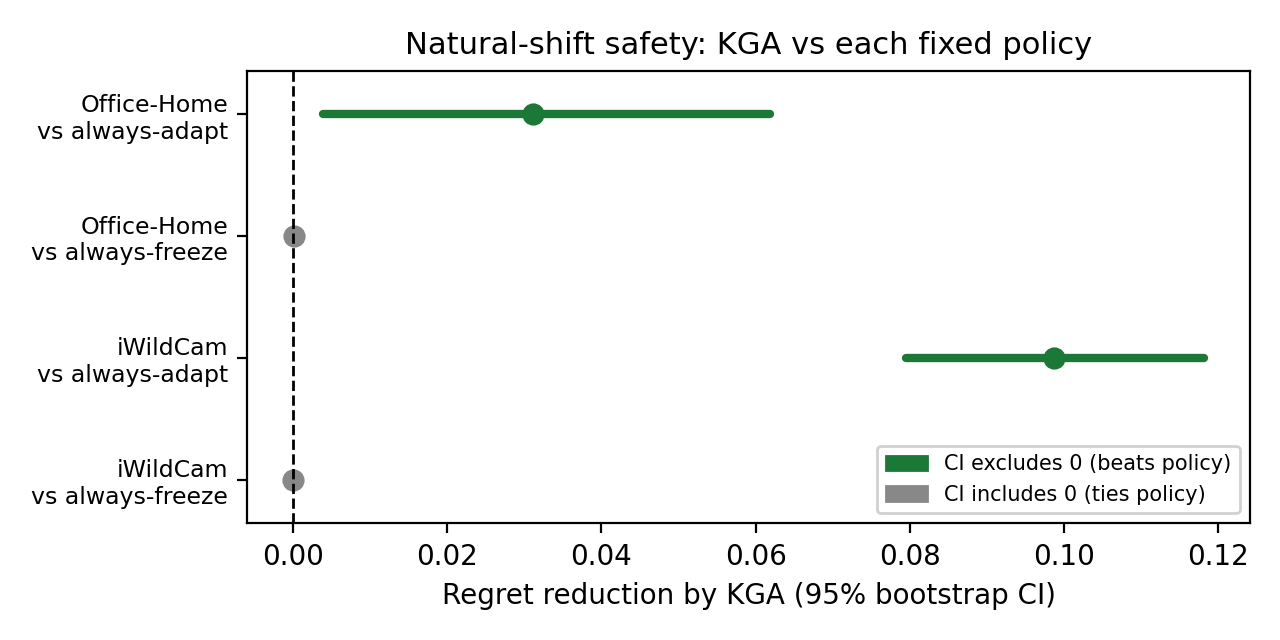
\includegraphics[width=0.96\linewidth]{figures/fig_natural_forest.png}
\caption{\textbf{Natural-shift action safety.} Positive values favor KGA. Office-Home
and iWildCam beat always-adapt but tie always-freeze under the corrected out-of-fold replay; the
intervals are paired held-out-condition bootstrap intervals from the saved OOF bootstrap lock
(App.~\ref{app:claim-artifact}).}
\label{fig:natural-forest}
\end{figure}

\paragraph{Multi-seed stability (Camelyon17).} The one natural-shift track with per-condition logs at
multiple seeds is Camelyon17 ($4$ seeds, $9$ composition-stress conditions/seed). Aggregating the
deployed per-seed decisions (locked per-seed artifacts, App.~\ref{app:claim-artifact}) shows the
no-harm outcome is \emph{candidate-dependent} and
stable only for the milder adapter (Table~\ref{tab:multiseed}): with Tent, KGA ties always-freeze and
beats always-adapt on all four seeds; with EATA the margin is inconclusive; and with the aggressive
helpful-dominated SAR arm KGA over-freezes (regret $0.0425$ versus always-adapt's $0.0002$).
The dominant fact about this table is structural, not empirical: at $n{=}9$ per seed the declared
exact-rank radius takes $k=\lceil10\cdot0.9\rceil=9=n$, so $\varepsilon$ is the \emph{maximum}
residual and $\mathrm{FA}_{\mathrm u}$ is forced to exactly $0$ for any data
(\S\ref{sec:fa-identity}). This is also the one table in the paper that cannot use the declared
leave-one-out-of-pool calibration: a pool of $8$ residuals needs $k=9$, which no finite radius
supplies, so the released library would return $\varepsilon=+\infty$ and abstain on all $36$ cells
(\S\ref{par:loo-pool}). We report the in-pool scoring and treat the
$\mathrm{FA}_{\mathrm u}$ column as void rather than as evidence. The $\mathrm{FA}_{\mathrm u}$ column of Table~\ref{tab:multiseed} therefore
carries no information, and the same is true of every $n\le12$ track in the panel. Under the archived
interpolated quantile the SAR arm's seed~$0$ showed $\mathrm{FA}_{\mathrm u}=1/9=0.111>\alpha$; we
record that exceedance rather than let the rule change hide it, and note that $1/9$ has a
Clopper--Pearson $95\%$ interval of $[0.003,0.429]$, so it is well inside binomial noise at this
sample size and is not evidence that the bound fails. The over-freezing itself has a simple cause: on
this track the realized radius is $0.07$--$0.09$ (SAR) and $0.15$--$0.37$ (Tent) against benefits of
order $10^{-3}$, so the interval essentially never excludes zero. Per-seed multi-seed replays for
iWildCam, Office-Home, and RxRx1 are single-run in the current artifacts and remain future work.

\begin{table}[t]\centering\footnotesize
\caption{\textbf{Multi-seed Camelyon17 (seeds $0$--$3$, $9$ conditions/seed).} Regret
mean$\pm$std across seeds, re-scored under the declared exact-rank radius. \textsc{ad} is the total
number of \textsc{adapt} decisions over $36$ cells. $\mathrm{FA}_{\mathrm u}$ is $0$ \emph{by
construction} at $n{=}9$ (\S\ref{sec:fa-identity}) and is shown only to make that point; it is not
evidence. Reproduced from the committed per-seed logs.}
\label{tab:multiseed}
\begin{tabular}{lccccl}
\toprule
candidate & KGA regret & adapt & freeze & \textsc{ad} & verdict \\
\midrule
Tent & $0.0201{\pm}0.0230$ & $0.1380$ & $0.0201$ & $0$ & ties freeze; never adapts \\
EATA & $0.0393{\pm}0.0252$ & $0.0417$ & $0.0424$ & $1$ & inconclusive \\
SAR  & $0.0425{\pm}0.0185$ & $0.0002$ & $0.0654$ & $5$ & over-freezes (helpful-dom.) \\
\bottomrule
\end{tabular}
\end{table}

\begin{table*}[t]\centering\scriptsize
\caption{\textbf{Uniform nine-track empirical panel.} Regrets are ordered as
KGA / always-adapt / always-freeze; lower is better; all rows use the declared exact-rank radius
(\S\ref{sec:exp-setup}). Fixed-policy comparisons are secondary. The ``\textsc{ad}'' column is the
number of \textsc{adapt} decisions, i.e.\ the number of opportunities the false-adapt guarantee had to
fail; rows marked $^{\dagger}$ have fewer than $10$ and their observed
$\mathrm{FA}_{\mathrm u}=0$ is uninformative (Table~\ref{tab:decision-accounting}). The final
column prevents a point estimate, a reconstructed summary, and a locked
multi-seed result from being presented as equivalent evidence.}
\label{tab:uniform-panel}
\setlength{\tabcolsep}{3.5pt}
\renewcommand{\arraystretch}{1.10}
\begin{tabular}{@{}p{0.14\textwidth}p{0.13\textwidth}cp{0.28\textwidth}p{0.15\textwidth}p{0.15\textwidth}@{}}
\toprule
Track & Evaluation unit & \textsc{ad} & Result & Decision interpretation & Evidence tier \\
\midrule
CIFAR-10-C stress & $5\times432$ per candidate & 1113 / 1244 & Tent: $0.0016/0.0079/0.1241$; EATA: $0.0013/0.0033/0.1314$; SAR withheld; $\mathrm{FA}_{\mathrm u}=0$, CP$_{95}$ upper on $\mathrm{FA}_{\mathrm c}$ $0.0027$ / $0.0024$ & selective routing; \textbf{the one powered track}. Cluster-robust beats-both for \emph{Tent only}: EATA's adapt-side CI includes zero once corruption is the cluster (Table~\ref{tab:cifar-cluster}) & locked (Tent/EATA; five raw seeds); SAR withheld (seed-0 aggregate non-reproducing) \\
ImageNet-C SAR & $27$ cells $\times$ $5$ seeds & 13 & $0.0289/0.0529/0.0319$ pooled; $\mathrm{FA}_{\mathrm u}=1/135=0.0074$, CP$_{95}$ $0.316$ & \textbf{point-estimate} no-harm vs.\ always-freeze; \emph{no} CI-supported beats-both at any legitimate unit & locked (5 seeds; $2/5$ seeds beat both, $3/5$ tie freeze exactly) \\
Camelyon17 OOD (EATA candidate) & genuine OOD test $n=18$ (support $n=36$) & n/r$^{\dagger}$ & $0.0000/0.0000/0.1381$; $\mathrm{FA}_{\mathrm u}=0$ & selects adapt-equivalent behavior & \textbf{not reproducible from the release}: the triple appears in no artifact on disk (App.~\ref{app:claim-artifact}) \\
iWildCam H v2 & held-out test $n=72$ & 1$^{\dagger}$ & $0.0041/0.1028/0.0041$; $\mathrm{FA}_{\mathrm u}=0$, CP$_{95}$ $0.950$ & no-harm, ties freeze; guarantee untested & locked (OOF bootstrap; single-run) \\
Office-Home M v2 & target test $n=35$ & 22 & $0.0157/0.0468/0.0158$; $\mathrm{FA}_{\mathrm u}=0$, CP$_{95}$ $0.127$ & no-harm, tiny point edge; CP bound is $1.3\times\alpha$ & locked (OOF no-harm only; LOO BB not promoted) \\
RxRx1 J & OOD test $n=60$ & 0$^{\dagger}$ & $0.0000/0.2531/0.0000$; $\mathrm{FA}_{\mathrm u}=0$ & freezes on every cell; guarantee untested & locked (real ckpt; single-run) \\
PACS & $3$ seeds $\times4$ LODO targets $\times18$ cells & 12 & mean regret $0.0431/0.0176/0.0446$; pooled $\mathrm{FA}_{\mathrm u}=2/216$, CP$_{95}$ on $\mathrm{FA}_{\mathrm c}$ $0.438$ & \textbf{worse than always-adapt} ($2.45\times$); all $12$ adapts come from one domain--seed cell, $2$ of them false & locked diagnostic null; no beats-both claim \\
ImageNet-R D & $4$ seeds $\times10$ backbones $\times12$ conditions & 0--46 & mean-across-backbone regret $0.0151/0.0064/0.0325$; per-backbone breakdown in Table~\ref{tab:imagenetr-backbone} & \textbf{worse than always-adapt on $7$ of $10$ backbones}; $4$ backbones have a $0\%$ harmful base rate & locked diagnostic null \\
CIFAR-10.1 K & cross-seed test $n=48$ & 18 & $0.0021/0.0190/0.0017$; $\mathrm{FA}_{\mathrm u}=0.167$ ($8/48$), $\mathrm{FA}_{\mathrm c}=0.444$ & fails transfer bar; no claim & locked diagnostic fail \\
\bottomrule
\end{tabular}
\end{table*}

\subsection{What an observed $\mathrm{FA}_{\mathrm u}=0$ does and does not establish}\label{sec:fa-identity}
Six of the nine panel rows report $\mathrm{FA}_{\mathrm u}=0$. Read naively that is a nine-track
confirmation of Theorem~\ref{thm:certificate}. It is not, for two separate reasons, and the honest
accounting makes the one genuinely strong track visible rather than burying it in a row of zeros.

\paragraph{(a) On in-\emph{sample} rank calibration, $\mathrm{FA}_{\mathrm u}\le\alpha$ cannot be
violated.} When $\varepsilon$ is the $k$-th order statistic of the same residual vector it is then
used to test, the number of residuals exceeding it is identically $n-k$. With
$k=\lceil(n{+}1)(1-\alpha)\rceil$ the miscoverage ceiling is therefore
$(n-k)/n$, a function of $n$ alone: $0.0972$ at $n{=}432$, $0.0370$ at $n{=}27$, and exactly $0$ at
$n\in\{9,12,18\}$, where $k=n$. All of these are below $\alpha{=}0.10$, so under in-sample
calibration ``$\mathrm{FA}_{\mathrm u}\le\alpha$'' holds for \emph{any} data whatsoever and is not a
measurement. We verified this ceiling is attained exactly on all $69$ shipped per-condition files.
The informative statistic is therefore $\mathrm{FA}_{\mathrm u}=0$ \emph{against that ceiling}, not
$\mathrm{FA}_{\mathrm u}\le\alpha$; and at $n\le18$ with $k=n$ (Camelyon17's
Table~\ref{tab:multiseed} cells, ImageNet-R conditions, PACS cells) the ceiling is $0$ and the
statistic carries no information at all.

This identity is exactly what the leave-one-out-of-pool calibration of \S\ref{par:loo-pool} breaks,
and breaking it is the point. Once cell $i$'s radius is fitted without cell $i$'s residual, nothing
forces the miscoverage count, and a nonzero $\mathrm{FA}_{\mathrm u}$ becomes \emph{possible}. It is
therefore informative that on CIFAR-10-C the count stays at $0$ over all $9{,}504$ committed cells
under the leave-one-out pool --- and equally informative that on ImageNet-C SAR it does not, moving
to $1/135$. A reader should read the CIFAR-10-C zero as a measurement and every $n\le18$ zero in the
panel as arithmetic.
For the same reason the realized calibration-set coverage figures ($0.898$ at $n{=}432$, $0.889$ at
$n{=}27$) are deterministic functions of $n$; earlier versions of our audit artifact attached Wilson
binomial intervals to them, which has no frequentist meaning, and those intervals have been removed.

\paragraph{(b) Where the guarantee is actually exercised.} A false-adapt bound is only tested by
\textsc{adapt} decisions. Table~\ref{tab:decision-accounting} reports the action composition of every
promoted row together with a one-sided Clopper--Pearson $95\%$ upper bound on the \emph{conditional}
rate $\mathrm{FA}_{\mathrm c}=\Pr[\Delta\le0\mid\textsc{adapt}]$ --- i.e.\ how much the observed zero
actually constrains anything. On CIFAR-10-C the bound is $0.0027$ from $1{,}113$ adapts. On ImageNet-C
SAR it is $0.316$ --- and there the observed conditional rate is not even $0$, it is $1/13$; on
Office-Home the bound is $0.127$; on iWildCam $0.950$. Three tracks (RxRx1 with $0$ adapts,
iWildCam with $1$, the D33 mechanism check with $9$) make fewer than $10$ \textsc{adapt} decisions and
we mark them \emph{guarantee untested}. The conclusion we draw is deliberately narrow: \textbf{the
certificate's safety guarantee is tested with real power on exactly one track, and there it holds}.

\begin{table}[t]\centering\small
\caption{\textbf{Action composition and the strength of the false-adapt evidence, per track.}
$\mathrm{FA}_{\mathrm u}$ is the marginal false-adapt rate the certificate bounds;
CP$_{95}$ is the one-sided Clopper--Pearson upper bound on the \emph{conditional} rate
$\mathrm{FA}_{\mathrm c}=\Pr[\Delta\le 0\mid\textsc{adapt}]$. $^{\dagger}$ fewer than $10$
\textsc{adapt} decisions: guarantee untested. Only CIFAR-10-C exercises the guarantee with power.}
\label{tab:decision-accounting}
\begin{tabular}{lccccccc}
\toprule
track & $N$ & \textsc{ad} & \textsc{fr} & \textsc{ab} & false & $\mathrm{FA}_{\mathrm u}$ & CP$_{95}$ \\
\midrule
CIFAR-10-C Tent & 2160 & 1113 & 358 & 689 & 0 & $0.0000$ & $\mathbf{0.0027}$ \\
CIFAR-10-C EATA & 2160 & 1244 & 130 & 786 & 0 & $0.0000$ & $\mathbf{0.0024}$ \\
ImageNet-C SAR & 135 & 13 & 15 & 107 & 1 & $0.0074$ & $0.3163$ \\
Office-Home M v2 & 35 & 22 & 12 & 1 & 0 & $0.0000$ & $0.1273$ \\
PACS (pooled) & 216 & 12 & 164 & 40 & 2 & $0.0093$ & $0.4381$ \\
iWildCam H v2$^{\dagger}$ & 72 & 1 & 60 & 11 & 0 & $0.0000$ & $0.9500$ \\
Camelyon17 OOD & 18 & --- & --- & --- & 0 & $0.0000$ & undef. \\
RxRx1 J$^{\dagger}$ & 60 & 0 & 60 & 0 & 0 & $0.0000$ & undef. \\
CIFAR-10.1 K & 48 & 18 & 24 & 6 & 8 & $0.1667$ & $0.6594$ \\
multimodal D33$^{\dagger}$ & 130 & 9 & 119 & 2 & 0 & $0.0000$ & $0.2831$ \\
\bottomrule
\end{tabular}

\vspace{2pt}
{\footnotesize Camelyon17's row is dashed because the promoted $n{=}18$ triple is not reproducible
from the release (App.~\ref{app:claim-artifact}); Office-Home, iWildCam, RxRx1 and CIFAR-10.1 counts
are $n_{\mathrm{test}}\times$ the promoted adapt rate, the CIFAR-10-C, ImageNet-C and PACS counts are
recomputed cell by cell.}
\end{table}

\subsection{Variance behind the panel means}\label{sec:panel-variance}
Three of the panel's aggregate rows average over a spread wide enough that the mean misdescribes the
track. We report the spread rather than the mean alone.

\paragraph{PACS.} The panel mean $0.0431$ is an average over $12$ domain--seed cells whose \textsc{KGA}
regret ranges from $0.00529$ to $0.15344$ (median $0.03616$, s.d.\ $0.03895$). The adapt rate is
\emph{zero} on $11$ of those $12$ cells: PACS's entire adaptation evidence is $12$ \textsc{adapt}
decisions taken on the single cell art\_painting/seed~$1$, and $2$ of the $12$ are false. That cell's
own $\mathrm{FA}_{\mathrm u}$ is $0.1111>\alpha$, and art\_painting/seed~$2$ abstains on all $18$
cells (decision coverage $0.0$). Pooled over all $216$ cells, $\mathrm{FA}_{\mathrm u}=2/216=0.0093$
(Wilson $95\%$ $[0.0025,0.0331]$), but $\mathrm{FA}_{\mathrm c}=2/12=0.167$ with a Clopper--Pearson
$95\%$ upper bound of $0.438$. PACS is a null in which \textsc{KGA} loses to always-adapt by
$2.45\times$; it is reported, not withdrawn.

\paragraph{ImageNet-R.} The mean-across-backbone row hides a reversal on most backbones
(Table~\ref{tab:imagenetr-backbone}). \textsc{KGA} is worse than always-adapt on $7$ of $10$
backbones, by up to $434\times$ (swin\_b) and $43.9\times$ (vit\_b\_16), and $4$ backbones have a
degenerate $0\%$ harmful base rate --- always-adapt is exactly oracle there, so any abstention costs
regret and the comparison is uninformative. On the two backbones with a substantial harmful base rate
(efficientnet\_b0 at $100\%$, swin\_t at $60.4\%$) \textsc{KGA} is better than always-adapt, which is
the regime map's prediction; the panel mean averages these opposite regimes together and should not
be read as a single verdict.

\begin{table}[t]\centering\footnotesize
\caption{\textbf{ImageNet-R per backbone} ($4$ seeds $\times12$ conditions each). Regrets
KGA / always-adapt / always-freeze; ``harm'' is the harmful base rate. Decomposition is from the
archived per-backbone scoring; the panel row above is the exact-rank aggregate. Under either quantile
rule \textsc{KGA}'s mean exceeds always-adapt's $0.0064$.}
\label{tab:imagenetr-backbone}
\begin{tabular}{lcccc}
\toprule
backbone & KGA & adapt & freeze & harm \\
\midrule
convnext\_base & $0.0000$ & $0.0000$ & $0.0693$ & $0.0\%$ \\
convnext\_tiny & $0.0207$ & $0.0015$ & $0.0221$ & $14.6\%$ \\
efficientnet\_b0 & $0.0000$ & $0.0506$ & $0.0000$ & $100.0\%$ \\
efficientnet\_b3 & $0.0186$ & $0.0000$ & $0.0501$ & $0.0\%$ \\
resnet101 & $0.0152$ & $0.0005$ & $0.0238$ & $8.3\%$ \\
resnet152 & $0.0088$ & $0.0000$ & $0.0421$ & $0.0\%$ \\
resnext101\_32x8d & $0.0059$ & $0.0000$ & $0.0520$ & $0.0\%$ \\
swin\_b & $0.0226$ & $0.0000$ & $0.0375$ & $2.1\%$ \\
swin\_t & $0.0043$ & $0.0106$ & $0.0047$ & $60.4\%$ \\
vit\_b\_16 & $0.0160$ & $0.0004$ & $0.0237$ & $6.2\%$ \\
\bottomrule
\end{tabular}
\end{table}

\paragraph{CIFAR-10-C stress grid.} Here the spread is small and it is worth saying so: per-seed
\textsc{KGA} regret is $0.001567$/$0.001631$/$0.001639$/$0.001440$/$0.001853$ for Tent
($\varepsilon$ coefficient of variation $0.030$) and $5/5$ seeds beat both fixed policies. EATA is
likewise $5/5$ with $\varepsilon$ c.v.\ $0.068$. The withheld SAR arm's $\varepsilon$ c.v.\ is
$0.390$, an order of magnitude larger, which is the quantitative form of the instability that put it
in quarantine (\S\ref{sec:cifar-stress}).

\subsection{Weak-Evidence and Negative Regimes}
ImageNet-R and CIFAR-10.1 remain diagnostics. Their outcomes are consistent with weak evidence,
low margin, estimator inadequacy, or calibration-transfer failure; they do not by themselves prove
structural non-identifiability. PACS is complete at three seeds but remains a null diagnostic in
which \textsc{KGA} loses to always-adapt.

\subsection{Physical-Study Pre-registration}
We preregister a two-phone physical package-inspection study with distinct source, calibration,
held-out, and replication sessions. The protocol, leakage checks, and outcome-free result templates
are provided in Appendix~\ref{app:edge-physical}. No physical result is claimed until fresh sessions
pass the repository's fail-closed publication gate; mock or reconstructed clips are never admissible
evidence.

\subsection{Constructed Heterogeneous Routing}\label{sec:constructed-routing}
The three-source OOF mixture combines separately calibrated Office-Home, iWildCam, and Camelyon17
conditions. It demonstrates routing value under a researcher-constructed heterogeneous stream, not
single-dataset natural-shift dominance or transfer to unseen shift types.

\begin{table}[t]\centering\scriptsize
\caption{\textbf{Primary numeric evidence used for empirical claims.} All rows use the declared
exact-rank radius. The three-source row is a constructed routing mixture, not a natural-transfer
result. ``CI utility'' means a paired bootstrap at the declared resampling unit whose interval
excludes zero against the named policy. ImageNet-C SAR has \emph{no} such policy: its entry is a
point estimate on both sides.}
\label{tab:primary-numeric}
\setlength{\tabcolsep}{3pt}
\begin{tabular}{@{}p{0.22\linewidth}p{0.14\linewidth}ccc p{0.21\linewidth}@{}}
\toprule
Track & Unit & KGA & Adapt & Freeze & Status \\
\midrule
CIFAR-10-C Tent & $5\times432$ & .0016 & .0079 & .1241 & locked; selective routing, $\mathrm{FA}_{\mathrm u}=0$ over $1113$ adapts; CI utility vs.\ both, \emph{cluster-robust} (Table~\ref{tab:cifar-cluster}) \\
CIFAR-10-C EATA & $5\times432$ & .0013 & .0033 & .1314 & locked; selective routing, $\mathrm{FA}_{\mathrm u}=0$ over $1244$ adapts; CI utility vs.\ freeze at every unit; vs.\ adapt \emph{only} at the cell/twin-pair unit --- clustering by corruption gives $[-0.0044,+0.0004]$ \\
ImageNet-C SAR & $27$ cond.\ (seed-avg.\ of $5$) & .0289 & .0529 & .0319 & locked (5 seeds); \textbf{no CI utility}: both condition-level gaps include zero under the promoted leave-one-out pool \\
Camelyon17 OOD & $n=18$ & .0000 & .0000 & .1381 & \textbf{not reproducible from release}; no artifact on disk contains this triple \\
RxRx1 J & $n=60$ & .0000 & .2531 & .0000 & locked; no-harm, but $0$ adapts --- guarantee untested \\
Three-source OOF mixture & $n=143$ & .0059 & .0632 & .0342 & locked; heterogeneous routing (constructed) \\
\bottomrule
\end{tabular}
\end{table}

\subsection{Consolidated Claim and Guarantee Accounting}\label{sec:guarantees}
\begin{center}
\scriptsize
\renewcommand{\arraystretch}{1.12}
\setlength{\tabcolsep}{4pt}
\begin{tabular}{@{}p{0.40\linewidth}p{0.14\linewidth}p{0.38\linewidth}@{}}
\toprule
Statement & Status & Requirement / observed \\
\midrule
Abstention needed in matched-evidence opposite-benefit worlds & theorem & stated model class \\
Label-free audit of $\beta$ is vacuous over the unrestricted class & theorem & Aud-A, App.~\ref{app:audit-short} \\
$\mathrm{FA}_u \le \alpha$ (unconditional false-adapt) & theorem & measurable marginal coverage; exchangeability/shift correction only justifies coverage \\
$\mathrm{FA}_u \le \alpha$ \emph{as measured on the grids} & \textbf{forced, not measured} & under in-sample rank calibration the ceiling is $(n{-}k)/n<\alpha$ for every $n$ used here (\S\ref{sec:fa-identity}) \\
$\mathrm{FA}_c \le \alpha$ (conditional false-adapt) & \textbf{not claimed} & CP$_{95}$ upper bound is $0.0027$ on CIFAR-10-C but $0.13$--$0.95$ elsewhere \\
An observed $\mathrm{FA}_{\mathrm u}$ exceedance exists in this paper & \textbf{yes, disclosed} & Camelyon17 SAR seed~$0$, $1/9=0.111$ under the archived interpolated rule; CP$_{95}$ interval $[0.003,0.429]$, i.e.\ inside binomial noise; PACS art\_painting seed~$1$, $2/18=0.111$ \\
Nine-track panel & \textbf{accounting} & sealed lock inventory (\texttt{NINE\_TRACK\_LOCK\_SEAL\_v1}); incomplete tracks stay diagnostic \\
Stress-grid action validity and routing utility (Tent/EATA) & locked & locked Protocol~A v1 stress grid; $6$ of $15$ corruptions, severities $\{1,5\}$ \\
CIFAR-10-C \emph{Tent} beats both, cluster-robustly & locked & adapt-gap CI excludes zero at all four units down to $6$ corruption clusters $[-0.0095,-0.0026]$; survives leave-one-corruption-out refit (Table~\ref{tab:cifar-cluster}) \\
CIFAR-10-C \emph{EATA} beats both, cluster-robustly & \textbf{not claimed} & adapt-gap CI includes zero at $12$ clusters $[-0.0048,+0.0004]$ and $6$ clusters $[-0.0044,+0.0004]$; two adverse corruption families. Point beats-both and the freeze-side CI stand \\
ImageNet-C SAR beats always-freeze & \textbf{point estimate only} & $0.0289$ vs.\ $0.0319$; under the promoted leave-one-out pool the condition-level CI $[-0.0085,+0.0038]$ and even the i.i.d.-135 CI $[-0.0079,+0.0036]$ include zero; $2/5$ seeds beat both \\
ImageNet-C SAR beats always-adapt & \textbf{point estimate only} & condition-level CI $[-0.076,+0.018]$ includes zero \\
Natural safety (RxRx1) & locked & held-out test artifacts; $0$ adapts, so the bound is untested \\
Natural safety (Camelyon17 $n{=}18$) & \textbf{unverifiable} & the promoted triple is in no released artifact \\
Office-Home and iWildCam OOF summaries & locked & OOF bootstrap seal (no-harm only; OH LOO BB not promoted) \\
Three-source mixed routing aggregate & locked & constructed OOF mixture, not transfer \\
Universal improvement & \textbf{not claimed} & impossible in general \\
No-harm on \emph{every} natural shift & \textbf{withdrawn} & holds on the four one-sided locked tracks; PACS and ImageNet-R lose to always-adapt \\
$\varepsilon$ estimates drift budget $\beta$ & \textbf{false} & $\beta$ is declared; $\varepsilon$ is empirical \\
\bottomrule
\end{tabular}
\end{center}

\section{Ablations and Sensitivity}\label{sec:ablations}
\subsection{Value of the Uncertainty Radius}
Table~\ref{tab:gates} isolates the radius: KGA without the radius has lower point regret but a higher empirical false-adapt rate, whereas the full certificate sacrifices coverage to eliminate observed harmful commitments on the locked grid. This comparison separates benefit-prediction quality from certification.

\subsection{Alpha, Evidence, Estimator, and Transfer Sensitivity}\label{sec:sens-ablations}
All ablations reuse the logged CIFAR-10-C stress evidence (per-condition $Z$ and true benefit $B$;
$432$ conditions/candidate, seed~0) and the deployed rule with an \emph{exact-rank} empirical residual radius
$\varepsilon=r_{(k)}$, $k=\lceil(n{+}1)(1-\alpha)\rceil$ (locked exact-rank ablation artifact with
input hashes, App.~\ref{app:claim-artifact}). At the deployed operating
point (Tent, $\alpha{=}0.10$) the harness reproduces the locked gate row of Table~\ref{tab:gates}
(regret $0.0017$, $\mathrm{FA}_{\mathrm u}{=}0$, adapt $0.51$, coverage $0.69$).

\textbf{(i) Safety level $\alpha$.} Sweeping $\alpha$ (Table~\ref{tab:abl-alpha}) trades decision
coverage for regret while holding $\mathrm{FA}_{\mathrm u}{=}0$ at every certified level; only the
radius-free variant breaks the guarantee ($\mathrm{FA}_{\mathrm u}=0.051$).
\textbf{(ii) Estimator.} Swapping the benefit regressor (Table~\ref{tab:abl-estimator}) leaves the
false-adapt guarantee intact: gradient boosting, random forest, and ridge all keep
$\mathrm{FA}_{\mathrm u}{\le}0.002$; a small MLP over-abstains on this small calibration set.
\textbf{(iii) Evidence family.} Dropping any single evidence family (frozen, adapted, change, drift,
or update) keeps regret in $[0.0015,0.0019]$ at $\mathrm{FA}_{\mathrm u}{=}0$: no single family is
load-bearing.
\textbf{(iv) Cross-adapter transfer.} Fitting the benefit model on one adapter and applying it to
another (Table~\ref{tab:abl-transfer}) \emph{breaks} the false-adapt bound in most directions
(SAR$\to$Tent $\mathrm{FA}_{\mathrm u}=0.25$), which is exactly why the deployed method refits per
adapter.
\textbf{(v) Drift budget $\beta$.} The population-frontier $\beta$ sweep is the synthetic
ground-truth validation of \S\ref{sec:synthetic}, kept distinct from the empirical radius
$\varepsilon$.

\begin{table}[t]\centering\footnotesize
\caption{Ablation (i): safety-level $\alpha$ sweep (exact-rank radius), CIFAR-10-C Tent ($n{=}432$).
$\mathrm{FA}_{\mathrm u}{=}0$ at every certified $\alpha$; only the radius-free row breaks it.}
\label{tab:abl-alpha}
\begin{tabular}{lcccc}
\toprule
$\alpha$ & regret$\downarrow$ & $\mathrm{FA}_{\mathrm u}$ & adapt & coverage \\
\midrule
$0.01$ & $0.0036$ & $0.000$ & $0.45$ & $0.48$ \\
$0.05$ & $0.0021$ & $0.000$ & $0.49$ & $0.63$ \\
$0.10$ & $0.0017$ & $0.000$ & $0.51$ & $0.69$ \\
$0.20$ & $0.0011$ & $0.000$ & $0.53$ & $0.74$ \\
no radius & $0.0004$ & $0.051$ & $0.68$ & $1.00$ \\
\bottomrule
\end{tabular}
\end{table}

\begin{table}[t]\centering\footnotesize
\caption{Ablation (ii): benefit estimator (exact-rank radius), CIFAR-10-C Tent ($\alpha{=}0.10$).
The radius keeps $\mathrm{FA}_{\mathrm u}{\approx}0$ regardless of estimator.}
\label{tab:abl-estimator}
\begin{tabular}{lcccc}
\toprule
estimator & regret$\downarrow$ & $\mathrm{FA}_{\mathrm u}$ & adapt & coverage \\
\midrule
gradient boosting & $0.0017$ & $0.000$ & $0.51$ & $0.69$ \\
random forest & $0.0017$ & $0.002$ & $0.51$ & $0.65$ \\
ridge (linear) & $0.0043$ & $0.000$ & $0.45$ & $0.47$ \\
small MLP & $0.0143$ & $0.000$ & $0.36$ & $0.36$ \\
\bottomrule
\end{tabular}
\end{table}

\begin{table}[t]\centering\footnotesize
\caption{Ablation (iv): cross-adapter transfer (exact-rank radius, $\alpha{=}0.10$). Transferring
one benefit model across adapters violates $\mathrm{FA}_{\mathrm u}{\le}\alpha$ in most
directions---per-adapter calibration is required.}
\label{tab:abl-transfer}
\begin{tabular}{lcccc}
\toprule
fit $\to$ apply & regret$\downarrow$ & $\mathrm{FA}_{\mathrm u}$ & adapt & coverage \\
\midrule
Tent $\to$ EATA & $0.0020$ & $0.000$ & $0.54$ & $0.63$ \\
EATA $\to$ Tent & $0.0010$ & $0.007$ & $0.55$ & $0.69$ \\
Tent $\to$ SAR & $0.0173$ & $0.125$ & $0.50$ & $0.72$ \\
EATA $\to$ SAR & $0.0236$ & $0.192$ & $0.57$ & $0.62$ \\
SAR $\to$ Tent & $0.0085$ & $0.255$ & $0.84$ & $0.84$ \\
SAR $\to$ EATA & $0.0027$ & $0.116$ & $0.75$ & $0.75$ \\
\bottomrule
\end{tabular}
\end{table}


\section{Discussion and Failure Modes}\label{sec:discussion}
\subsection{Why Natural Shifts Mainly Produce No-Harm}
A single natural benchmark is often one-sided: adaptation helps almost everywhere or harms almost everywhere. In the first case, always-adapt is already near-oracle; in the second, always-freeze is near-oracle. A three-way router gains a strict margin over both fixed policies only when helpful and harmful conditions coexist and the evidence distinguishes them. Natural no-harm results and mixed-regime wins are therefore different operating points of the same decision geometry.

\subsection{Four Sources of Abstention}
Not every abstention has the same interpretation. \emph{Structural non-identifiability} means opposite-benefit worlds share the same admissible evidence law. \emph{Finite-sample uncertainty} means the sign is identifiable in principle but the interval still crosses zero. \emph{Estimator inadequacy} means the chosen model fails to extract an available signal. \emph{Calibration failure} means a development relationship does not transfer to deployment. We distinguish these causes throughout the evaluation rather than treating every null result as evidence of structural unknowability.

\subsection{Operational Failure Modes}
Table~\ref{tab:failure-modes} maps each deployment failure to a diagnostic and a safe response.
\begin{table}[t]\centering\scriptsize
\caption{Deployment failures, diagnostics, and safe responses.}
\label{tab:failure-modes}
\begin{tabular}{@{}p{0.28\linewidth}p{0.30\linewidth}p{0.32\linewidth}@{}}
\toprule
Failure & Diagnostic & Safe response \\
\midrule
Calibration transfer fails & support/residual audit & recalibrate, widen radius, or abstain \\
True drift exceeds $\beta$ & external domain monitoring & revise class/budget; freeze meanwhile \\
Evidence out of support & distance or density check in $Z$-space & abstain \\
Adapter/checkpoint changed & configuration hash mismatch & require recalibration \\
Batch too small & minimum-size rule & wait for more data or freeze \\
Continual state accumulates error & checkpoint/stream monitor & rollback to last certified state \\
Missing/invalid evidence & schema and numerical validation & freeze \\
\bottomrule
\end{tabular}
\end{table}

\subsection{When to Deploy K-Bound}
K-Bound is most valuable when harmful updates are plausible, the cost of a bad commit is high, a frozen fallback is available, and historical or structural information supports calibration. It is less useful when adaptation is uniformly benign, when no credible drift class or calibration set exists, or when the candidate update cannot be evaluated and rolled back safely.

\section{Limitations}\label{sec:limits}

\medskip
\textbf{Scope of empirical decision evidence.} On the stress grid \textsc{KGA} exercises selective adapt/freeze/abstain behavior for Tent/EATA
(Table~\ref{tab:decisive}); CIFAR-10-C SAR is withheld. On ImageNet-C the pattern flips by candidate---Tent/EATA
are robust while SAR collapses and \textsc{KGA} retains low regret under a mechanism-faithful re-run
(Table~\ref{tab:imagenetc-faithful}). Per-corruption CIFAR-10-C and helpful natural shifts are
insurance regimes, not policy wins.

\textbf{Real-shift scope.} The uniform panel deliberately distinguishes three outcomes, and the
no-harm claim covers only the first. Camelyon17
genuine OOD and RxRx1 are no-harm results: KGA ties the better fixed policy at
zero observed false-adapt --- with the caveats that Camelyon17's promoted $n{=}18$ triple is not
reproducible from the release and that RxRx1 makes zero \textsc{adapt} decisions, so neither
exercises the guarantee. Office-Home and iWildCam are locked from their out-of-fold bootstrap seal
(App.~\ref{app:claim-artifact}; Office-Home promotes OOF no-harm only; LOO beats-both is not claimed);
iWildCam makes one \textsc{adapt} decision. PACS and ImageNet-R are completed, locked null
diagnostics in which \textsc{KGA} \emph{loses} to always-adapt --- by $2.45\times$ on PACS and on $7$
of $10$ ImageNet-R backbones --- and CIFAR-10.1 is a locked diagnostic fail. We state the losses in
the limitations section as well as the results section because the abstract of an earlier version of
this paper asserted no-harm across ``every natural distribution shift we test'', which these three
tracks contradict.
The three-source mixture is a constructed routing aggregate; it is not a transfer result and does not
change the per-dataset conclusion.

\textbf{Theory and calibration.} The conformal radius assumes exchangeable calibration pairs;
sign bracketing without structure is impossible (Theorems~\ref{lem:nonid}
and~\ref{thm:headline}; Appendix~\ref{app:theory-full}). \textsc{KGA}'s value scales with how often catastrophic,
detectable harm occurs, not with universal accuracy gains. On helpful-dominated shifts the
resulting near-\emph{tie} with always-adapt reflects the certificate abstaining rather than
committing harmful updates: \textsc{KGA} approximately matches the better policy, at most paying a
small abstention cost when it declines a helpful but uncertifiable update, so the value proposition
is conditional, like insurance against detectable harm.
\emph{Setting $\beta$.} The budget is \emph{declared}, not estimated from unlabeled data---and
provably so: label-free audits of $\beta$ are vacuous over the unrestricted class
(Appendix~\ref{app:audit-short}). It can, however, be \emph{audited}: a labeled audit budget, a
Lipschitz-transport assumption, or an unknown-direction index-drift assumption yields a computed
upper bound with finite-sample validity, at the price of the named side information. Absent an audit, $\beta$ is fixed from domain knowledge,
historical dev-to-deployment gaps, or an explicit stress envelope.
The choice $\beta{=}0$ is the strongest zero-drift assumption and may be reported only as a plug-in baseline; it is not an assumption-free or conservative default. When no credible bound is justifiable, the population frontier cannot certify robustness to calibration drift, and the safe operational response is to abstain or freeze. Larger $\beta$ widens the abstain band monotonically, trading decision coverage for robustness.

\textbf{Detectability and transfer.} ImageNet-R is a weak, split-specific evidence regime:
no candidate survives both comparisons across four seeds. CIFAR-10.1 fails the
cross-seed certificate bar ($\mathrm{FA}_{\mathrm u}=0.167$ and descriptive
$\mathrm{FA}_{\mathrm c}=0.444$). These are useful boundary cases,
not failed headline experiments: they show that a low-margin signal should not be promoted merely
because one split or one candidate looks favorable.

\textbf{Theory limits versus empirical limits.} Some abstention is compatible with the population
frontier, whereas baseline faithfulness, seed count, estimator quality, and replay status are ordinary
empirical limitations requiring further validation. Tying always-adapt on a helpful-dominated shift is the no-harm
guarantee \emph{holding}: one cannot beat an oracle that is already always-adapt. Declining
ImageNet-R is consistent with a weak-evidence, low-margin regime; the null result does not by itself
establish structural non-identifiability under Theorem~\ref{thm:headline} (it could also reflect weak
evidence, poor benefit estimation, or calibration-transfer failure). Abstention in the structurally
ambiguous closed band prevents a uniformly sound strict commitment over the declared class. Empirical
abstention, however, may instead stem from an overly wide radius or a weak estimator and therefore does
not establish that a tested shift lies in that structural band. Richer label-free evidence may improve
benefit estimation and reduce avoidable abstention, while better-justified or more data-efficient
calibration can narrow finite-sample uncertainty; neither removes the population limitation without
strengthening the declared assumptions or evidence.

\textbf{Baseline scope and recomputation.} On the ImageNet-C SAR configuration, the
committal confidence gate adapts on harmful cells while KGA abstains on the low-margin band. The
POEM/AETTA comparison is complete only for protocol-matched ports; official implementations remain
future baseline work. The Office-Home/iWildCam summaries have a separate saved recomputation lock,
but no external-lab replication. PACS and ImageNet-R are completed registered diagnostics and are
retained as null/weak-evidence results rather than tuned into wins. The frozen external procedure is
documented in \texttt{INDEPENDENT\_REPLICATION\_PROTOCOL.md}. Abstention lowers \emph{decision} coverage
but never withholds a prediction: it retains the frozen fallback $f_0$.

\begin{center}\fbox{\parbox{0.95\linewidth}{\small
\textbf{What we do not claim.} Universal accuracy gains; adapter selection by test regret;
multicandidate routes with violated false-adapt bounds; or wins on helpful-dominated shifts
where always-adapt is already oracle-optimal.}}
\end{center}

\section{Reproducibility}\label{sec:repro-main}
\subsection{Artifacts and Result Lineage}
All locked/reconciled rows in Tables~\ref{tab:uniform-panel}--\ref{tab:primary-numeric} link to
saved raw cells or seed aggregates in the released repository, with two documented exceptions: the
Camelyon17 $n{=}18$ triple, whose reconciliation directory is absent from the release, and the
Office-Home and iWildCam promoted regrets, whose named record files are absent while two other
scorings of the same track survive and disagree (App.~\ref{app:claim-artifact}). Those three rows
are marked \emph{not reproducible from the release} rather than \emph{locked}. Provisional rows are
retained only to document completed evidence and the required replay; they are not reused as headline
claims. The core certificate module is packaged as an installable module in the same repository.
\ifanon
\emph{Anonymity note.} For double-blind review the repository link and the \texttt{CITATION.cff}
author block are withheld; the release itself is not anonymized and must be redacted before an
anonymous submission, not merely described as anonymous.
\fi
\subsection{Formal Verification Scope}
The repository contains a kernel-checked Lean~4 formalization of indexed algebraic,
finite-decision, measure-containment, and conditional uniform-rank results, with no
\texttt{sorry}, \texttt{admit}, or project-defined axioms. It checks frontier sufficiency, all three
deterministic branches, algebraic witnesses for the closed and open bands, both zero-versus-strict
boundary witnesses, and the marginal false-adapt/false-freeze implication once coverage is assumed.
The current development does not formalize the target-law witness construction, equality of its
induced evidence laws, membership of those laws in $\mathcal C_\beta$, realization of the algebraic
witnesses by measurable target laws, distributional frontier necessity or pointwise maximality,
risk alignment, multiclass identifiability, calibration transfer, or a
general exchangeable-process lift. These clauses are proved only in the manuscript; compilation of
the mapped helper declarations is not described as kernel verification of the complete paper theorem. The
implementation theorem uses the same exact rank rule as the current clean-split scorer; historical
benchmark artifacts produced with an interpolated empirical quantile are not presented as
kernel-certified split-conformal experiments. Machine-checked learning-theory results are an
emerging area---Lean formalizations of generalization-error bounds exist~\cite{sonoda2025lean}---and
to our knowledge machine-checked conformal-coverage results remain uncommon; no priority claim is
made.

\subsection{Claim-to-Support Map}
\begin{table*}[t]\centering\scriptsize
\caption{\textbf{Claim-to-support map.} ``Theorem'' means proved in the manuscript; Lean coverage is
limited to the inventory described above. ``Empirical'' and ``diagnostic'' claims are restricted to
the named saved artifacts and protocols.}
\label{tab:claim-status}
\begin{tabular}{@{}p{0.20\textwidth}p{0.075\textwidth}p{0.22\textwidth}p{0.22\textwidth}p{0.20\textwidth}@{}}
\toprule
Claim & Type & Exact requirement & Evidence location & Caveat \\
\midrule
Interior matched-evidence impossibility & theorem & $\beta>0$, $|M|<\beta$, declared class contains the constructed worlds & Thm.~\ref{lem:nonid}; App.~\ref{app:theory-full} & Opposite nonzero benefits are an interior result only. \\
Closed-band abstention & theorem & Strict three-way soundness over $|\gamma|\le\beta$ & Prop.~\ref{prop:closed-band} & Boundary is zero-versus-strict ambiguity, not opposite signs. \\
Strict-commitment frontier & theorem & Declared drift class and risk alignment & Thm.~\ref{thm:headline} & Uniform strict commitment, not universal sign recovery. \\
Marginal $\mathrm{FA}_{\mathrm u}$ certificate & theorem & $\Pr(|\widehat\Delta-\Delta|\le\varepsilon)\ge1-\alpha$ & Thm.~\ref{thm:certificate}; Lean inventory & Does not control conditional $\mathrm{FA}_{\mathrm c}$. \\
CIFAR-10-C mixed-regime action validity & empirical & Five-seed Tent/EATA raw decisions, action rates, false-adapt, and paired CIs & Table~\ref{tab:decisive}; empirical audit manifest & SAR is withheld after a replay mismatch and contributes no evidence. \\
ImageNet-C authoritative result & empirical & 27 cells $\times$ 5 seeds, SAR candidate, pooled seed-averaged paired bootstrap & Table~\ref{tab:imagenetc-faithful}; Table~\ref{tab:imagenetc-ci-unit} & Under the promoted leave-one-out pool neither condition-level gap excludes 0; $2/5$ seeds beat both, $3/5$ tie freeze exactly. \\
Natural no-harm results & empirical & Reconciled OOF or locked held-out artifacts & Tables~\ref{tab:uniform-panel}--\ref{tab:primary-numeric} & One-sided regimes mainly exercise the adapt or freeze branch. \\
Controlled multimodal routing & empirical & Pre-registered $13\times10$ injected-corruption grid & App.~\ref{app:d33}; \texttt{KB-CLAIM-027} & Mechanism confirmation, not a natural multimodal benchmark. \\
POEM/AETTA comparison & empirical & Same logged stress cells and protocol-matched ports & Table~\ref{tab:headtohead-poem-aetta} & Not official implementations. \\
Constructed heterogeneous mixture & empirical & Researcher-constructed three-source routing aggregate & Sec.~\ref{sec:constructed-routing} & Not unseen-shift transfer. \\
Universal improvement & diagnostic & No supporting requirement is declared & Sec.~\ref{sec:limits} & Explicitly not claimed. \\
Universal accuracy improvement & diagnostic & Would require a different objective and task-specific held-out evidence & Natural-shift tables & Explicitly not claimed. \\
Real-camera study & pending & Fresh preregistered held-out sessions and raw logs & pre-registration templates & Templates are not evidence. \\
\bottomrule
\end{tabular}
\end{table*}

\section{Conclusion}
K-Bound reframes test-time adaptation as a validity and safety decision---whether to adapt at all---rather than an unconditional update, and contributes the missing decision layer: a label-free adapt/freeze/abstain certificate with a controlled false-adapt rate. The central object is the target benefit $\Delta=R_T(f_0)-R_T(f_a)$. Over a declared drift-budget class, a strict adapt or freeze commitment is uniformly supportable if and only if the observable disagreement-region margin exceeds the declared budget; on $|M|\le\beta$, abstention is the maximal sound three-way action under the paper's strict-decision semantics. We are explicit about which half of that ``iff'' carries content: sufficiency is interval arithmetic on a decomposition we defined, while necessity rests on a construction of two admissible target laws with identical label-free evidence and opposite nonzero benefits---the same construction that makes label-free auditing of the budget itself vacuous.

KGA operationalizes this principle with a label-free benefit estimate and a pre-calibrated uncertainty radius. The resulting controller commits the candidate only when the interval excludes zero, retains the frozen model when harm is certified, and otherwise abstains from changing state. Across the benchmark panel the primary outcome is a safety one, and it is scoped: on the four one-sided natural tracks with locked held-out artifacts (Camelyon17, iWildCam, Office-Home, RxRx1) KGA ties the better fixed policy at zero observed false adaptation; on PACS, ImageNet-R, and CIFAR-10.1 it is a conservative null or fails the declared transfer bar, and those three are reported as such rather than removed from the panel. Controlled mixed regimes---including the pre-registered two-view multimodal check of Appendix~\ref{app:d33}---additionally exercise all three actions and confirm, as a secondary mechanism check, that the certificate can beat both fixed policies where helpful and harmful conditions coexist and are separable by the evidence. The safety guarantee itself is exercised with genuine statistical power on one track only: the CIFAR-10-C stress grid, at $1{,}113$ \textsc{adapt} decisions and zero false adaptations. Weak or non-transferable evidence produces abstention or remains diagnostic rather than being promoted as a win.

The broader implication is that an adaptation system should expose two components: an update mechanism and a validity layer that decides whether the update is supportable under the available evidence and assumptions. Strengthening K-Bound therefore requires not only better adapters, but also richer risk-aligned evidence, more defensible calibration across shifts, explicit drift-budget auditing, and reproducible deployment semantics.

